% Target venue: Journal of Machine Learning Research (single-column full-length).
% Compiled with a JMLR-compatible article layout; swap in jmlr2e.sty at submission.
\documentclass[11pt]{article}
\usepackage[margin=1.15in]{geometry}
\usepackage{amsmath,amssymb,amsthm,mathtools}
\usepackage{booktabs}
\usepackage{graphicx}
\usepackage{url}
\usepackage{longtable}
\usepackage{pdflscape}
\usepackage{algorithm}
\usepackage{algpseudocode}
\usepackage[numbers,sort&compress]{natbib}

\newtheorem{theorem}{Theorem}
\newtheorem{lemma}{Lemma}
\newtheorem{proposition}{Proposition}
\newtheorem{corollary}{Corollary}
\newtheorem{assumption}{Assumption}
\theoremstyle{remark}
\newtheorem{remark}{Remark}
\newcommand{\R}{\mathbb{R}}
\newcommand{\E}{\mathbb{E}}
\newcommand{\dd}{\mathrm{d}}
\newcommand{\TV}{\mathrm{TV}}
\graphicspath{{figs/}}
\sloppy

\title{Learned Transport Atlases for Exact,\\ Gradient-Free Production MCMC}
\author{Bhum Soonjun\\[2pt]
\small Draft manuscript prepared for the Journal of Machine Learning Research.\\
\small Code, benchmark artifacts, and reproduction scripts accompany the submission.}
\date{}

\begin{document}
\maketitle

\begin{abstract}
We present \emph{Pathfinder Mixture-Referenced Hamiltonian Monte Carlo}
(PMR-HMC), a Markov chain Monte Carlo sampler that is fast, efficient, and
exact: its production phase makes \emph{zero} calls to the target-gradient
oracle and exactly \emph{one} call to the target-density oracle per
transition, while its invariant law is the target posterior for any fixed
surrogate---a property that follows from the invariant-kernel construction
and is additionally checked end-to-end by simulation-based calibration.
Inference is split into a finite warm-up that learns geometry and a frozen
production phase that exploits it. Warm-up constructs a \emph{transport
atlas}: a mixture reference $q=\sum_k w_kq_k$ whose components push a
standard normal through invertible chart maps---affine Laplace charts,
composed quadratic shears, conditional log-scale charts, polar (winding)
charts, hierarchical location--scale charts, Student-$t$ charts, and
sinh-arcsinh triangular charts---so that each chart's Jacobian is
absorbed into the exactly evaluated component density and the latent
dynamics remain exactly harmonic. Production alternates
chart-conditional trajectories, integrated in closed form and corrected
by a single target-density Metropolis test, with independence proposals
from a defensive mixture; the resulting independence kernel is
uniformly ergodic whenever the proposal dominates the target. We prove exactness for arbitrary fixed cached
forces, for non-injective winding charts via preimage-summed densities with
Jacobian-weighted branch sampling, and for Student-$t$ charts via an exact
scale-mixture auxiliary. Under exact-atlas conditions we prove three
production \emph{complexity separations}: target-oracle cost per
effective sample is $O(1)$ in the condition number $\kappa$, where
gradient-based HMC requires $\Theta(\sqrt\kappa)$ gradient calls per
effective sample; $O(1)$ in the ambient dimension $d$ at fixed residual
dimension, where optimal scaling forces $\Theta(d^{1/4})$; and $O(1)$ in
the separation between posterior modes, where local-flow samplers mix in
time exponential in barrier height. We further give acceptance bounds
separating surrogate from discretization error.
Empirically, \emph{production} target-oracle cost per effective sample
is flat in condition
number $\kappa\in[10^2,10^5]$ where NUTS scales as $\Theta(\sqrt\kappa)$,
flat in dimension $d\in[50,200]$ at fixed residual dimension, and flat in
mode separation where NUTS ceases to switch modes while reporting high
within-mode effective sample size. On a 37-posterior benchmark drawn
from \emph{posteriordb}, judged against gold-standard reference draws
under a symmetric accuracy gate, PMR-HMC is the best of a ten-method
panel---diagonal- and dense-mass NUTS, Pathfinder-initialized dense
NUTS, ChEES, MCLMC, and four flow-based samplers (TESS,
flow-based independence MH, a flowMC-style hybrid, NeuTra)---on 34 of
37 posteriors, with median advantages, over rows where both samplers
pass the gate, of $38\times$ over diagonal NUTS, $4.1\times$ over
dense NUTS, $10$--$12\times$ over ChEES and MCLMC (which pass on only
$11$ and $19$ of 37 rows), and $29$--$95\times$ over the flow-based
samplers, which fail the accuracy gate outright on the large majority
of posteriors (cross-seed rank-$\widehat R\le1.05$ everywhere except
the two disclosed accuracy failures); a curated 30-target controlled
stress panel that deliberately retains every known failure family
localizes where the method wins and loses, with every accuracy failure
attributable to a named missing chart class or warm-up budget and the
efficiency losses concentrated on smooth, well-scaled targets. A
production boundary study localizes the failure of any single global
map at $d\approx600$ via a measured per-coordinate fidelity law, and a
delayed-rejection hybrid restores gate-passing quality there at
$2$--$5\times$ the speed of the production NUTS baseline (single-seed
prototype). A native C production
kernel attains $0.13$--$385\,\mu$s per draw; end-to-end wall clock
crosses over in PMR-HMC's favor beyond a median budget of
$\approx4{,}500$ effective samples.
\end{abstract}

\paragraph{Keywords} Markov chain Monte Carlo; Hamiltonian Monte Carlo;
transport maps; variational reference; Bayesian computation; surrogate
modeling; exact sampling.

\section{Introduction}\label{sec:intro}
The computational bottleneck of applied Bayesian inference is the oracle:
each evaluation of the log posterior or its gradient may traverse a large
data set, a differential-equation solver, or a production decision model.
Gradient-based samplers in the Hamiltonian Monte Carlo (HMC) family
\citep{duane1987,neal2011}, and the No-U-Turn Sampler (NUTS)
\citep{hoffman2014} in particular, purchase their mixing by spending
gradients \emph{continuously}: every leapfrog step of every trajectory
queries $\nabla U$, and the number of steps needed per effective sample
grows with the condition number of the posterior covariance
\citep{neal2011,langmore2019}, with dimension \citep{beskos2013}, and,
without bound, with the separation between posterior modes
\citep{mangoubi2018}.

This paper develops the converse decomposition: \emph{first remove the
structure that a quasi-Newton, optimization-driven warm-up can explain;
then approximate only what remains}. A finite warm-up learns a mixture
reference $q$ built from invertible chart maps fitted to optimizer paths
and pilot states. The residual
\begin{equation}
R(x)\;=\;U(x)+\log q(x),\qquad U=-\log\tilde\pi,
\label{eq:residual}
\end{equation}
is then (a) nearly constant wherever the atlas fits and (b) typically
low-dimensional where it does not. Production sampling requires no
gradient-oracle calls at all: the Gaussian part of the latent dynamics is
integrated in closed form, cached residual forces supply the correction,
and a single call to the target-density oracle at the trajectory endpoint
restores exactness through a Metropolis test. A calibrated independence
branch mixes between modes at a rate independent of barrier height.
Figure~\ref{fig:hero} summarizes the pipeline.

The central object is the \emph{transport atlas}: a mixture
$q(x)=\sum_{k=1}^Kw_k\,q_k(x)$ whose components are push-forwards of a
standard normal through chart maps $T_k$. Because the augmented target
factorizes so that each chart's Jacobian cancels against the exactly
evaluated $q_k$ (Section~\ref{sec:construction}), the latent dynamics
conditional on a chart are \emph{exactly harmonic regardless of how
nonlinear the chart is}. Chart design thereby becomes a modeling language:
a quadratic shear linearizes banana-shaped ridges; a conditional log-scale
chart linearizes funnels; a polar chart with a wrapped-Gaussian angle
circulates ring-shaped level sets; and a hierarchical location--scale chart
reproduces, automatically, the non-centered reparameterization that
practitioners apply by hand
\citep{papaspiliopoulos2007,betancourt2015}. All charts are learned from
warm-up data by closed-form estimators.

\subsection{Contributions}
\begin{enumerate}
\item An exact transport-atlas kernel
  (Sections~\ref{sec:construction}--\ref{sec:exact}) whose production
  transitions use zero gradient-oracle calls and one target-density-oracle
  call, with proofs of invariance for arbitrary fixed cached forces; for
  non-injective (winding) charts via preimage-summed densities with
  Jacobian-weighted branch sampling; and for Student-$t$ charts via an
  exact Gamma-auxiliary Gibbs step, developed over the full augmented
  space.
\item Seven learned chart classes (Section~\ref{sec:charts}) with
  consistent closed-form detection estimators, recovering analytic
  transports at machine precision on their canonical geometries.
\item Theory (Section~\ref{sec:theory}): uniform ergodicity of the mixed
  kernel \emph{conditional on} a bounded target-to-proposal ratio;
  acceptance bounds separating surrogate error from $O(h^2)$
  discretization error; and a cost model with amortization break-even.
\item \textbf{Three complexity separations against known baseline
  scalings} (Theorem~\ref{thm:sep}): under exact-atlas conditions we
  \emph{prove} the PMR-HMC side---production target-oracle cost per
  effective sample $O(1)$ in condition number, $O(1)$ in ambient
  dimension at fixed residual dimension, and $O(1)$ in mode
  separation---and contrast it with the established scalings of
  gradient-based samplers ($\Theta(\sqrt\kappa)$ trajectory length,
  $\Theta(d^{1/4})$ steps, exponential barrier mixing), which are
  cited, not re-proved here. Arithmetic cost is accounted separately
  (Table~\ref{tab:cost}); the experiments show that \emph{learned}
  atlases realize all three separations to close approximation.
\item A reproducible empirical study (Section~\ref{sec:experiments}):
  measured cost flat in $\kappa$, in $d$, and in mode separation; a
  37-posterior benchmark drawn from \emph{posteriordb}
  \citep{magnusson2024} with gold-reference judging and a full inclusion
  table, on which PMR-HMC is the accuracy-gated best of a ten-method
  panel---dense-mass and Pathfinder-initialized NUTS, ChEES-HMC
  \citep{hoffman2021}, MCLMC \citep{robnik2023}, TESS, flow-based
  independence MH, a flowMC-style hybrid, and NeuTra---on 34 of 37
  posteriors; a curated 30-target stress panel retaining every known
  failure family; decomposition ablations attributing the gains among
  atlas, dynamics, and independence branch; a production advertising
  model; and a native C kernel measured in both wall-clock regimes.
\item An end-to-end implementation check by simulation-based calibration
  \citep{talts2018}; exactness itself follows from the construction, and
  SBC serves as a pipeline audit.
\end{enumerate}

\begin{figure}[t]
\centering
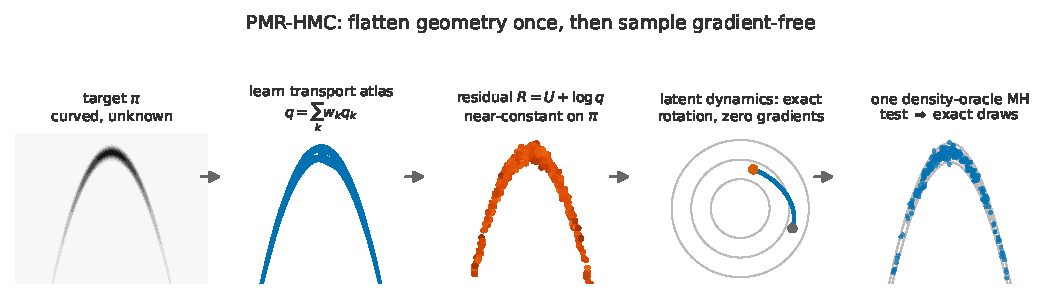
\includegraphics[width=\textwidth]{hero.pdf}
\caption{\textbf{The method in one picture.} A curved posterior (left) is
explained by a learned transport atlas $q$ (chart contours, blue; affine
charts, vermillion); the residual $R=U+\log q$ then flattens, so the
latent dynamics reduce to an exactly integrable harmonic rotation
requiring no gradients, and a single target-density Metropolis test per
transition restores exactness. Warm-up learns the atlas once; production
never adapts.}
\label{fig:hero}
\end{figure}

\section{Related Work}\label{sec:related}
\textbf{HMC and adaptive trajectories.} HMC \citep{duane1987,neal2011}
suppresses random-walk behavior via Hamiltonian flow; NUTS
\citep{hoffman2014}, with adaptive mass matrices \citep{stan2017}, defines
the practical state of the art. ChEES-HMC \citep{hoffman2021} replaces the
recursive tree with a learned trajectory length; MEADS \citep{hoffman2022}
and microcanonical samplers \citep{robnik2023,robnik2024} alter the
underlying dynamics. All retain per-step gradient evaluation.
Optimal-scaling theory gives step size $h=\Theta(d^{-1/4})$ on product
targets \citep{beskos2013} and trajectory length $\Theta(\sqrt\kappa)$
under ill-conditioning \citep{neal2011,langmore2019}.

\textbf{Geometry-aware and transport-preconditioned MCMC.} Riemannian HMC
\citep{girolami2011} adapts to local curvature at cubic per-step cost.
Split HMC \citep{shahbaba2013} integrates a Gaussian component exactly;
pCN and $\infty$-HMC \citep{beskos2011,cotter2013} do so against a
Gaussian reference measure. Transport-map MCMC
\citep{parno2018,marzouk2016} and NeuTra-HMC
\citep{hoffman2019} precondition dynamics with learned maps;
normalizing-flow-assisted samplers learn global proposals
\citep{albergo2019,gabrie2022}. Our construction differs in three
respects: the reference is a \emph{mixture of heterogeneous charts} whose
Jacobians are absorbed into an exactly evaluated density; the latent
dynamics remain harmonic in \emph{every} chart; and the learned objects
are deliberately low-capacity---charts fitted by closed-form regressions,
with all residual error absorbed by an exact accept step rather than by
model capacity.

\textbf{Surrogates and delayed acceptance.} Surrogate-gradient HMC
\citep{rasmussen2003,strathmann2015,zhang2017}, delayed-acceptance MCMC
\citep{christen2005,sherlock2017}, and learned kicks inside reversible
compositions \citep{neklyudov2020,levy2018,song2017} established that
approximate dynamics with exact correction preserve the target. We use
this map-level exactness (Lemma~\ref{lem:involution}) but approximate only
$\nabla\log(\pi/q)$ in its active subspace, which is empirically far
easier than the full score.

\textbf{Optimization-initialized inference.} Pathfinder \citep{zhang2022}
constructs Gaussian approximations along L-BFGS \citep{liu1989} paths;
Laplace-type methods \citep{rue2009} exploit curvature at the mode. We
extend the idea from initialization to a full sampling kernel: optimizer
paths supply chart candidates, surrogate anchors, and free residual
training data.

\textbf{Independence samplers and ergodicity.} Uniform ergodicity of the
independence sampler under a bounded target-to-proposal ratio is classical
\citep{mengersen1996,tierney1994,roberts2004}; adaptation requires care
\citep{andrieu2008,roberts2007}. Our global branch inherits the classical
guarantee because adaptation is frozen; the defensive heavy-tailed
component follows importance-sampling practice
\citep{hesterberg1995,owen2000}.

\textbf{Benchmarking.} We adopt \emph{posteriordb} \citep{magnusson2024}
with its gold-standard reference draws, rank-normalized effective sample
size \citep{vehtari2021}, and simulation-based calibration
\citep{talts2018}.

\section{Setting and Oracle Model}\label{sec:setting}
Let $\tilde\pi=e^{-U}$ be an unnormalized density on $\R^d$ with $U$
continuously differentiable. The sampler may query two \emph{target
oracles}: the density oracle $x\mapsto U(x)$ and the gradient oracle
$x\mapsto(U(x),\nabla U(x))$. Throughout, ``one density evaluation''
means one call to the target-density oracle; mixture densities,
responsibilities, chart inverses, and cached forces are internal
arithmetic, itemized separately in Table~\ref{tab:cost}. For scalar
summaries we convert a gradient call to $c_g$ density-units and report
$c_g=2.5$ (a typical reverse-mode factor), together with raw counts and a
sensitivity analysis over $c_g\in[1,4]$
(Section~\ref{sec:oracleacct}); Hessian evaluations are charged $d$
gradient calls. Efficiency is reported as target-oracle units per
effective sample, using rank-normalized bulk ESS \citep{vehtari2021}
minimized over coordinates; accuracy as maximum standardized moment error
against analytic truth or gold reference draws.

\section{The Transport-Atlas Construction}\label{sec:construction}
\subsection{Chart-augmented target}
Let $T_k:\R^d\to\R^d$, $k=1,\dots,K$, be differentiable maps, each either
a diffeomorphism or a countably-sheeted covering map
(Section~\ref{sec:winding}), and let $\varphi$ denote the standard normal
density. Define component densities by the push-forward
\begin{equation}
q_k(x)\;=\;\sum_{z\in T_k^{-1}(x)}
\frac{\varphi(z)}{\bigl|\det DT_k(z)\bigr|},
\qquad
q=\sum_{k=1}^K w_kq_k,
\label{eq:qk}
\end{equation}
with weights $w\in\Delta_{K-1}$ and responsibilities
$r_k(x)=w_kq_k(x)/q(x)$. When a fiber $T_k^{-1}(x)$ is countably
infinite (the winding chart), the implementation truncates the branch
sum at $|k_w|\le K_w$; the discarded mass is a Gaussian tail,
$\sum_{|k_w|>K_w}\varphi_1\!\bigl((\theta+2\pi k_w)/c\bigr)\le
2\,\Phi\!\bigl(-(2\pi K_w-\pi)/c\bigr)$, below double precision for
the fitted $c$ at $K_w{=}64$, so the truncated $q_k$ is the density
actually used---consistently in evaluation and in branch
sampling---and exactness is preserved for the truncated reference.

\begin{lemma}[Augmentation]\label{lem:aug}
$\bar\pi(x,k)\coloneqq\pi(x)\,r_k(x)$ is a probability density on
$\R^d\times[K]$ with $x$-marginal $\pi$. For a diffeomorphic $T_k$, the
conditional law of $z=T_k^{-1}(x)$ given $k$ under $\bar\pi$ satisfies
\begin{equation}
\bar\pi(z\mid k)\;\propto\;
\exp\!\Bigl(-\tfrac12\lVert z\rVert^2-R\bigl(T_k(z)\bigr)\Bigr),
\label{eq:latenttarget}
\end{equation}
with $R$ as in \eqref{eq:residual}.
\end{lemma}
\begin{proof}
$\sum_kr_k\equiv1$ gives the marginal claim. For the conditional, change
variables $x=T_k(z)$:
\begin{align*}
\bar\pi(z\mid k)
&\propto\pi(T_kz)\,r_k(T_kz)\,\bigl|\det DT_k(z)\bigr|\\
&=\frac{w_k\,\pi(T_kz)}{q(T_kz)}\;q_k(T_kz)\,\bigl|\det DT_k(z)\bigr|.
\end{align*}
For a diffeomorphism the last factor equals $\varphi(z)$ by
\eqref{eq:qk}, while $\pi/q=e^{-R}/Z$; together these yield
\eqref{eq:latenttarget}.
\end{proof}

The essential point is that the Jacobian of an arbitrarily nonlinear chart
cancels against the exactly evaluated $q_k$: conditional on $k$ the latent
prior is exactly $\mathcal N(0,I)$, all non-Gaussian structure is
concentrated in $R\circ T_k$, and the phase-space target
$\rho_k(z,p)\propto e^{-H_k}$ with
\begin{equation}
H_k(z,p)=\tfrac12\lVert z\rVert^2+\tfrac12\lVert p\rVert^2
+R\bigl(T_k(z)\bigr)
\label{eq:H}
\end{equation}
is dominated by an exactly solvable harmonic oscillator whenever the atlas
fits: Figure~\ref{fig:ressurf} shows the residual over the posterior
draws of a banana target spanning $22$ nats under the best single
Gaussian but $6$ nats under the learned atlas---the flattening that
cached, gradient-free dynamics require. Exact integration of a Gaussian reference
part is the split-HMC mechanism \citep{shahbaba2013} and, in
reference-measure form, the preconditioned-Crank--Nicolson rotation of
function-space samplers \citep{beskos2011,cotter2013}; fiber-summed
densities for non-injective maps appear in surjective normalizing flows
\citep{nielsen2020}. What is new here is their combination into a
\emph{learned heterogeneous mixture atlas} with Gibbs chart resampling,
winding and heavy-tailed charts inside an exact kernel, and cached
zero-gradient residual forces selected by the error-knee criterion.

\subsection{Production kernel}\label{sec:kernel}
Algorithm~\ref{alg:prod} summarizes production. One local transition
consists of four exactly specified maps. First, the chart is refreshed and
the state lifted:
\begin{equation}
k\sim r_\cdot(x),\qquad z=T_k^{-1}(x),\qquad p\sim\mathcal N(0,I).
\end{equation}
Second, the latent pair is propagated by $L$ steps of the symmetric
splitting $\Psi_h=\mathcal K_{h/2}\circ\mathcal O_h\circ\mathcal K_{h/2}$
with factors
\begin{align}
\mathcal O_h(z,p)&=\bigl(z\cos h+p\sin h,\;-z\sin h+p\cos h\bigr),
\label{eq:rot}\\
\mathcal K_a(z,p)&=\bigl(z,\;p-a\,\hat f_k(z)\bigr),
\label{eq:kick}
\end{align}
the exact harmonic rotation and a momentum kick by the cached residual
force. No discretization error is incurred in any direction the atlas
explains. Third, the endpoint $y=T_k(z_L)$ is accepted with probability
\begin{equation}
\alpha_{\mathrm{loc}}
=1\wedge\exp\bigl(H_k(z_0,p_0)-H_k(z_L,p_L)\bigr),
\label{eq:mh}
\end{equation}
which makes the transition's single call to the target-density oracle (in
$R(y)$); the current state's $U(x)$ and $\log q(x)$ are cached from its
own acceptance. Fourth, with probability $p_g$ the transition instead
draws a global independence proposal from the defensive mixture
\begin{equation}
g=(1-\epsilon)\,q+\epsilon\,t_\nu(\cdot;\mu_0,\Sigma_0),
\label{eq:defensive}
\end{equation}
accepted with the independence ratio
\begin{equation}
\alpha_{\mathrm{glob}}
=1\wedge\frac{\tilde\pi(y)\,g(x)}{\tilde\pi(x)\,g(y)}.
\label{eq:imh}
\end{equation}
The trajectory time is randomized, $T\sim\mathrm{Unif}[0.35\pi,0.65\pi]$
(centered near $\pi/2$, at which the pure rotation maps $z\mapsto p$, so
successive draws of an atlas-explained target are independent) to avoid
harmonic resonances; the momentum flip that makes the proposal an
involution (Lemma~\ref{lem:involution}) is omitted from
Algorithm~\ref{alg:prod} because the momentum is fully refreshed each
transition. Default settings used in all experiments: $p_g=0.2$,
defensive weight $\epsilon=0.1$ with $\nu=4$, dual-averaging target
$0.7$, and step cap $L_{\max}=48$. All quantities are frozen before
production.

\begin{algorithm}[t]
\caption{Production transition (frozen atlas)}\label{alg:prod}
\begin{algorithmic}[1]
\State \textbf{given} state $x$ with cached $U(x),\log q(x)$
\If{$\mathrm{Unif}(0,1)<p_g$}
  \State $y\sim g$; accept w.p.\ \eqref{eq:imh}
    \Comment{one target-density call}
\Else
  \State $k\sim r_\cdot(x)$;\; $z\gets T_k^{-1}(x)$
    \Comment{branch/auxiliary sampled if required}
  \State $p\sim\mathcal N(0,I)$;\; $T\sim\mathrm{Unif}[T_-,T_+]$,
    $L=\mathrm{round}(T/h)\wedge L_{\max}$
  \State $(z',p')\gets\Psi_{T/L}^{\,L}(z,p)$ \Comment{cached forces only}
  \State $y\gets T_k(z')$; accept w.p.\ \eqref{eq:mh}
    \Comment{one target-density call}
\EndIf
\end{algorithmic}
\end{algorithm}

\subsection{Cached residual forces}\label{sec:surrogate}
Two force models are precomputed per chart from warm-up anchors
$\{(z_i,f_i)\}$, $f_i=J_k(z_i)^\top\nabla R(T_kz_i)$, both acting in the
\emph{active subspace}: with $C=\sum_if_if_i^\top$ and $V\in\R^{d\times s}$
its top-$s$ eigenvectors, $\hat f_k(z)=V\hat g(V^\top z)$.

\paragraph{Compact scalar radial-basis energy.} With Wendland kernel
$\psi(r)=(1-r)_+^4(4r+1)$ \citep{wendland1995}, farthest-point centers
$c_j$ and bandwidths $\ell_j$,
\begin{equation}
\widehat R_k(u)=\sum_{j=1}^M a_j\,
\psi\!\left(\frac{\lVert u-c_j\rVert}{\ell_j}\right),
\qquad u=V^\top z,
\label{eq:rbf}
\end{equation}
fitted by ridge least squares jointly on residual values and projected
gradients, with closed-form gradient
\begin{equation}
\nabla\widehat R_k(u)
=-20\sum_j\frac{a_j}{\ell_j^2}
\Bigl(1-\frac{\lVert u-c_j\rVert}{\ell_j}\Bigr)_{\!+}^{3}(u-c_j).
\label{eq:rbfgrad}
\end{equation}
The force is conservative and vanishes smoothly outside the union of
supports: the trust region is the energy's own support, so far from data
the dynamics revert to exact harmonic motion---surrogate failure degrades
acceptance, never correctness.

\paragraph{Local-affine nearest-neighbor field.} Alternatively, with
per-anchor Jacobians $B_i$ from local least squares and kernel weights
$\omega_i(u)$ over the $m$ nearest anchors,
\begin{equation}
\hat g(u)=\lambda(u)\sum_{i\in\mathcal N_m(u)}
\omega_i(u)\bigl[f_i+B_i(u-u_i)\bigr],
\label{eq:affine}
\end{equation}
with a smooth distance gate $\lambda(u)\to0$ beyond the anchor set. This
field is not conservative; by Lemma~\ref{lem:involution} exactness is
unaffected. The per-chart model (\eqref{eq:rbf}, \eqref{eq:affine}, or
zero force) is selected on held-out data (Section~\ref{sec:estimators}).

\begin{figure}[t]
\centering
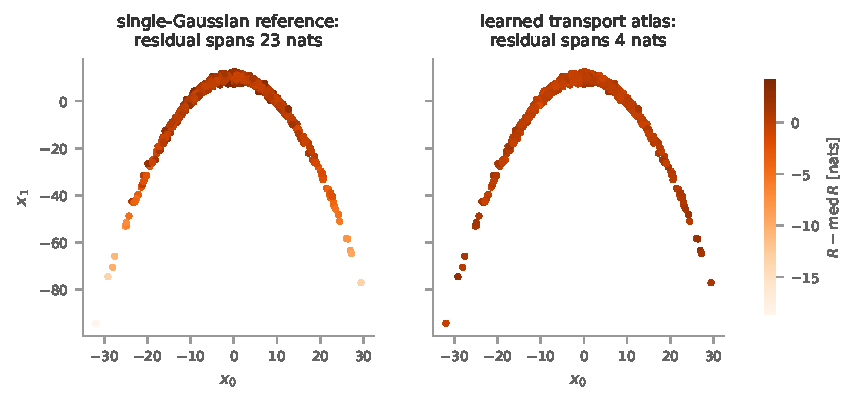
\includegraphics[width=.92\textwidth]{residual_surface.pdf}
\caption{\textbf{What the atlas buys.} The residual $R=U+\log q$
evaluated at posterior draws of the banana target ($d{=}20$), colored on
a common scale. Left: under a moment-matched single Gaussian, $R$ varies
by $22$ nats along the ridge---no cached force model can track this
without gradients. Right: under the learned transport atlas the same
draws span $6$ nats, most of it in the extreme arm tips.}
\label{fig:ressurf}
\end{figure}

\section{Exactness}\label{sec:exact}
\begin{lemma}[Volume-preserving involution]\label{lem:involution}
For any fixed measurable $\hat f_k$, the splitting
$\Psi=\mathcal K_{h/2}\mathcal O_h\mathcal K_{h/2}$ is volume preserving,
and with momentum flip $F(z,p)=(z,-p)$ the proposal
$T_{\mathrm{prop}}=F\Psi^L$ is a volume-preserving involution.
\end{lemma}
\begin{proof}
$\mathcal K_a$ is a $p$-shear at fixed $z$ (unit Jacobian); $\mathcal O_h$
is orthogonal. From $F\mathcal K_aF=\mathcal K_a^{-1}$ and
$F\mathcal O_hF=\mathcal O_h^{-1}$ we get $F\Psi F=\Psi^{-1}$, hence
$(F\Psi^L)^2=\mathrm{id}$. Conservativeness of $\hat f_k$ is not required.
\end{proof}

\begin{theorem}[Invariance]\label{thm:exact}
Fix the atlas, weights, caches, $h$, and $p_g$. The kernel that (i)
resamples $k\sim r_\cdot(x)$, (ii) refreshes $p$, (iii) proposes
$T_{\mathrm{prop}}$ and accepts with $1\wedge e^{-\Delta H_k}$, and (iv)
with probability $p_g$ instead performs the independence step, preserves
$\bar\pi$ and hence $\pi$.
\end{theorem}
\begin{proof}
Step (i) is a Gibbs update of $k\mid x$ under $\bar\pi$
(Lemma~\ref{lem:aug}). Conditional on $k$, the phase-space target
$\rho_k\propto e^{-H_k}$ is preserved by a Metropolis test with a
volume-preserving involutive proposal
\citep{tierney1994,neklyudov2020}: the flow rate
\begin{equation*}
\rho_k(s)\,\Bigl(1\wedge\frac{\rho_k(Ts)}{\rho_k(s)}\Bigr)
=\min\bigl\{\rho_k(s),\,\rho_k(Ts)\bigr\}
\end{equation*}
is symmetric under $s\leftrightarrow Ts$ because $\lvert\det DT\rvert=1$
and $T^2=\mathrm{id}$. Momentum refresh preserves the Gaussian marginal;
the independence step targets the $x$-marginal directly; a
state-independent mixture of invariant kernels is invariant.
\end{proof}

\subsection{Winding charts}\label{sec:winding}
The polar chart maps
\begin{equation}
(z_r,z_\theta)\;\mapsto\;
(R+\sigma_rz_r)\bigl(\cos cz_\theta,\;\sin cz_\theta\bigr),
\label{eq:polar}
\end{equation}
acting as the identity on the remaining coordinates, and is deliberately
non-injective: $z_\theta$ and $z_\theta+2\pi/c$ share an image, so a
wrapped, nearly uniform angular law covers the circle and the harmonic
flow in $z_\theta$ circulates it (Figure~\ref{fig:winding}).

\begin{figure}[t]
\centering
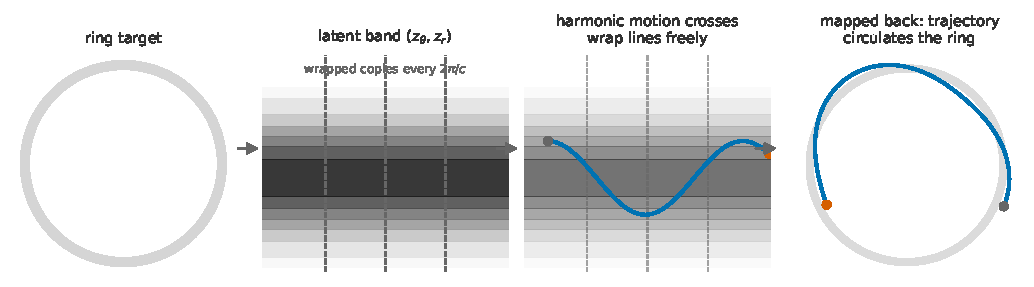
\includegraphics[width=\textwidth]{winding.pdf}
\caption{\textbf{The winding chart, step by step.} A closed ridge is
unwrapped into a latent band on which the angular coordinate repeats
every $2\pi/c$; harmonic motion travels freely along the band, and
mapping back yields a trajectory that circulates the ring---the geometry
that defeats arc-by-arc mixtures of local charts. Exactness under the
non-injective map requires the fiber-summed density \eqref{eq:qk} and
branch-sampled inversion \eqref{eq:branch}
(Lemma~\ref{lem:winding}).}
\label{fig:winding}
\end{figure}

\begin{lemma}[Winding exactness]\label{lem:winding}
Let $T_k$ be a covering map with countable fibers and $q_k$ defined by
\eqref{eq:qk}. Suppose the chart inversion samples the branch
$Z\in T_k^{-1}(x)$ with probability
\begin{equation}
\Pr(Z=z)\;=\;
\frac{\varphi(z)/\lvert\det DT_k(z)\rvert}
{\sum_{z'\in T_k^{-1}(x)}\varphi(z')/\lvert\det DT_k(z')\rvert}.
\label{eq:branch}
\end{equation}
Then the kernel of Theorem~\ref{thm:exact} remains $\bar\pi$-invariant.
For charts whose Jacobian determinant is constant on each fiber---as for
the polar chart \eqref{eq:polar}, where
$\lvert\det DT_k\rvert=\sigma_rc\,\lvert R+\sigma_rz_r\rvert$ depends on
the fiber only through the common radius---rule \eqref{eq:branch} reduces
to sampling $\propto\varphi(z)$. A deterministic (principal-branch)
inversion need not preserve $\bar\pi$ (and measurably breaks
calibration in the ablation of Section~\ref{sec:negative}).
\end{lemma}
\begin{proof}
Define the latent density
$\rho(z\mid k)\propto\varphi(z)\,e^{-R(T_kz)}$ on all of $\R^d$. Its
push-forward through $T_k$ has density
\begin{equation*}
\sum_{z\in T_k^{-1}(x)}
\frac{\varphi(z)\,e^{-R(x)}}{\lvert\det DT_k(z)\rvert}
\;=\;q_k(x)\,e^{-R(x)}
\;\propto\;\frac{q_k(x)\,\pi(x)}{q(x)},
\end{equation*}
the $\bar\pi$-conditional of $x$ given $k$; and at fixed $x$ the fiber
conditional of $z$ is proportional to
$\varphi(z)/\lvert\det DT_k(z)\rvert$, since $e^{-R(x)}$ is
fiber-constant. Sampling \eqref{eq:branch} is therefore an exact draw of
$z\mid(x,k)$, and the latent Metropolis step preserves
$\rho(\cdot\mid k)$ as in Theorem~\ref{thm:exact}. Under a deterministic
branch rule, a trajectory whose endpoint wraps is paired, on reversal,
with a starting point different from the forward endpoint's latent
representative, so the involution pairing of Lemma~\ref{lem:involution}
fails and detailed balance with it.
\end{proof}

\begin{remark}
Equation~\eqref{eq:branch} is the general statement; implementations that
sample $\propto\varphi$ alone are exact only for fiber-constant
Jacobians. Our polar chart satisfies this; a winding chart with
fiber-varying determinant must use \eqref{eq:branch}.
\end{remark}

\subsection{Student-$t$ charts}\label{sec:tcharts}
Heavy-tailed targets defeat Gaussian atlases: $\pi/q$ is unbounded and
both branches stall. The scale-mixture identity
\begin{equation}
t_\nu(x;\mu,\Sigma)=\int_0^\infty
\mathcal N\!\bigl(x;\mu,\Sigma/\lambda\bigr)\,
\Gamma\!\bigl(\lambda;\tfrac\nu2,\tfrac\nu2\bigr)\,\dd\lambda
\label{eq:scalemix}
\end{equation}
restores the construction; we give the complete augmented-space argument.

\begin{lemma}[$t$-chart exactness]\label{lem:tchart}
Let chart $k$ be a $t$-chart with parameters $(\mu_k,\Sigma_k,\nu)$ and
component density $q_k=t_\nu(\cdot;\mu_k,\Sigma_k)$ inside
\eqref{eq:qk}--\eqref{eq:residual}. Define the augmented target on
$(x,k,\lambda)$ by
\begin{equation}
\bar\pi(x,k,\lambda)
=\pi(x)\,r_k(x)\,p_k(\lambda\mid x),
\qquad
p_k(\lambda\mid x)
=\Gamma\!\Bigl(\lambda;\;\frac{\nu+d}{2},\;
\frac{\nu+\delta_k(x)}{2}\Bigr),
\label{eq:taug}
\end{equation}
with $\delta_k(x)=\lVert L_k^{-1}(x-\mu_k)\rVert^2$. Then:
(i) the $(x,k)$-marginal of \eqref{eq:taug} is the chart-augmented target
of Lemma~\ref{lem:aug}; (ii) $p_k(\lambda\mid x)$ is the exact
conditional of the auxiliary in \eqref{eq:scalemix}, so drawing it is a
Gibbs step; (iii) conditional on $(k,\lambda)$, the change of variables
$z=\sqrt\lambda\,L_k^{-1}(x-\mu_k)$ yields
\begin{equation}
\bar\pi(z\mid k,\lambda)\;\propto\;
\exp\!\Bigl(-\tfrac12\lVert z\rVert^2
-R\bigl(T_{k,\lambda}(z)\bigr)\Bigr),
\qquad
T_{k,\lambda}(z)=\mu_k+\frac{L_kz}{\sqrt\lambda},
\label{eq:tlatent}
\end{equation}
with the same residual $R=U+\log q$ (the marginal-$t$ density $q_k$
inside $q$). Consequently the kernel that per transition draws
$\lambda\sim p_k(\cdot\mid x)$ and then applies the local Metropolis step
of Theorem~\ref{thm:exact} in the chart $T_{k,\lambda}$ preserves
\eqref{eq:taug} and hence $\pi$.
\end{lemma}
\begin{proof}
(i) is immediate since $p_k$ integrates to one. For (ii), Bayes' rule
under \eqref{eq:scalemix} gives
\begin{equation*}
p(\lambda\mid x)\;\propto\;
\mathcal N\!\bigl(x;\mu_k,\Sigma_k/\lambda\bigr)\,
\Gamma\!\bigl(\lambda;\tfrac\nu2,\tfrac\nu2\bigr)
\;\propto\;
\lambda^{\frac{\nu+d}{2}-1}
e^{-\frac{\lambda}{2}(\nu+\delta_k(x))},
\end{equation*}
the stated Gamma law. For (iii), substitute $x=T_{k,\lambda}(z)$ in
\eqref{eq:taug}:
\begin{align*}
\bar\pi(z\mid k,\lambda)
&\propto
\pi(x)\,\frac{w_kq_k(x)}{q(x)}\,p_k(\lambda\mid x)\,
\Bigl|\det\tfrac{L_k}{\sqrt\lambda}\Bigr|\\
&\propto
e^{-R(x)}\,q_k(x)\,p_k(\lambda\mid x)\,
\lambda^{-d/2}\lvert L_k\rvert.
\end{align*}
By \eqref{eq:scalemix} and (ii),
$q_k(x)\,p_k(\lambda\mid x)
=\mathcal N(x;\mu_k,\Sigma_k/\lambda)\,
\Gamma(\lambda;\frac\nu2,\frac\nu2)$, and
$\mathcal N(x;\mu_k,\Sigma_k/\lambda)\,\lambda^{-d/2}\lvert L_k\rvert
\propto\varphi(z)$ up to $z$-free factors; all remaining
$\lambda$-dependence is $z$-free and cancels in $\Delta H$. Thus
\eqref{eq:tlatent} holds, the affine-chart argument of
Theorem~\ref{thm:exact} applies conditionally on $(k,\lambda)$, and the
composition of the Gibbs step with the Metropolis step preserves
\eqref{eq:taug}. The chart-refresh step uses the \emph{marginal} $t$
density inside $r_k$, so step (i) of Theorem~\ref{thm:exact} is
unchanged.
\end{proof}

\subsection{Global branch: conditional uniform ergodicity}
\begin{theorem}[Uniform ergodicity under tail dominance]\label{thm:ue}
\emph{Assume} $M\coloneqq\sup_x\pi(x)/g(x)<\infty$. Then the production
kernel $P$ satisfies $P(x,\cdot)\ge(p_g/M)\,\pi(\cdot)$ and hence
\begin{equation}
\lVert P^n(x,\cdot)-\pi\rVert_{\TV}\;\le\;\bigl(1-p_g/M\bigr)^n
\quad\text{for all }x.
\label{eq:uebound}
\end{equation}
\end{theorem}
\begin{proof}
The two-case argument of \citet{mengersen1996} gives the pointwise
minorization
\begin{equation*}
g(y)\,\Bigl(1\wedge\frac{\pi(y)\,g(x)}{\pi(x)\,g(y)}\Bigr)
\;\ge\;\frac{\pi(y)}{M};
\end{equation*}
mixing with the local kernel scales it by $p_g$, and \eqref{eq:uebound}
follows from the full-space minorization \citep{roberts2004}.
\end{proof}

\begin{remark}[The assumption is not automatic]
The defensive $t_\nu$ component in \eqref{eq:defensive} is designed to
make $M$ finite and moderate for targets whose tails are dominated by
$t_\nu$, but tail dominance is an \emph{assumption} to be checked, not a
consequence of adding a $t$ component: a target with heavier or otherwise
non-dominated tails need not satisfy it. When it holds, mode mixing
costs $O(1)$ proposals per switch independent of barrier height, in
contrast to the exponential mixing of local samplers on multimodal
targets \citep{mangoubi2018}; empirically
(Figure~\ref{fig:scaling}c) NUTS records zero switches beyond separation
four while our switch rate is flat.
\end{remark}

\section{Learned Chart Classes}\label{sec:charts}
Each class is fitted by a closed-form estimator
(Section~\ref{sec:estimators}); each recovers its canonical geometry,
verified as machine-precision unit tests: under the analytic funnel
transport the residual spread is $\operatorname{sd}(R)\approx10^{-15}$
with acceptance $1.000$; the analytic ring chart attains acceptance
$0.97$.

Figure~\ref{fig:catalogue} shows each class acting on its canonical
geometry: the defining property of every chart is that its latent view
(right column) is standard normal, so the harmonic dynamics of
Section~\ref{sec:kernel} apply unchanged.

\begin{figure}[p]
\centering
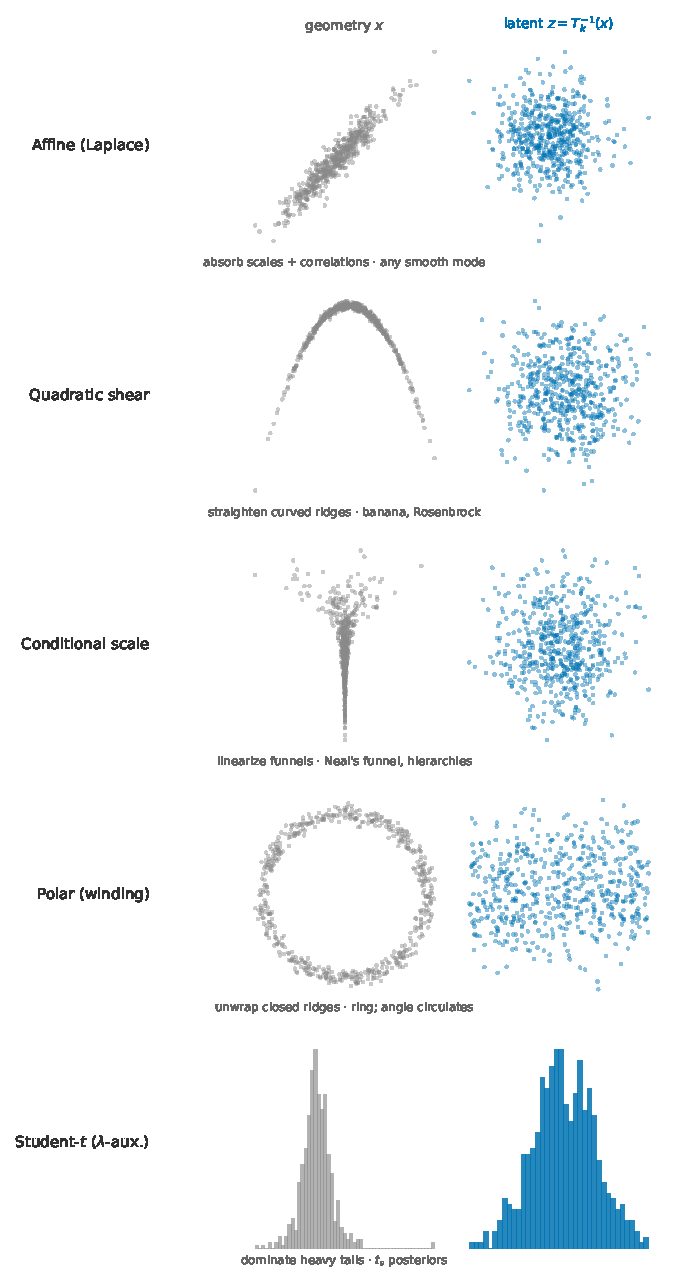
\includegraphics[width=.62\textwidth]{catalogue.pdf}
\caption{\textbf{Chart catalogue.} Five of the seven learned chart
classes (rows; the hierarchical location--scale and sinh-arcsinh
triangular classes act like the conditional-scale row with a
coordinate-valued location and a skew/tail-warped marginal,
respectively) each map
its canonical geometry (left, gray) to an approximately standard-normal
latent view (right, blue). Affine charts absorb scales and correlations;
quadratic shears straighten curved ridges (banana, Rosenbrock);
conditional-scale charts linearize funnels; polar charts unwrap closed
ridges; Student-$t$ charts Gaussianize heavy tails conditionally on the
scale auxiliary $\lambda$. Purpose and canonical example are annotated
under each row.}
\label{fig:catalogue}
\end{figure}

\paragraph{Affine (Laplace) charts.} $T_k(z)=\mu_k+L_kz$, with $\Sigma_k$
an $\lvert$eigenvalue$\rvert$-clipped inverse Hessian at
evidence-selected points of L-BFGS paths \citep{zhang2022,liu1989}.

\paragraph{Composed quadratic shears.} Over disjoint driver--target
pairs,
\begin{equation}
x_{t_j}\;\mapsto\;x_{t_j}
+\gamma_j\bigl((x_{d_j}-\mu_{d_j})^2-m_j\bigr),
\label{eq:shear}
\end{equation}
with unit determinant, detected by the partial-$R^2$ statistic
\eqref{eq:partialr2} and peeled iteratively so that simultaneous
curvatures compose into one chart. The Rosenbrock density is exactly a
composed-shear Gaussian; the estimator recovers every pair coefficient
($\hat\gamma\in[0.999,1.004]$, truth $1$) from valley-spanning data.

\paragraph{Conditional log-scale charts.} With driver coordinate $v$,
\begin{equation}
x_i=\mu_i+\sigma_i
\exp\!\bigl(\tfrac12(\alpha_i+\beta_i(v-\bar v))\bigr)\,z_i,
\label{eq:scalechart}
\end{equation}
fitted by \eqref{eq:scalereg}; exact for Neal's funnel \citep{neal2003}
at $\beta\equiv1$.

\paragraph{Polar (winding) charts.} Equation~\eqref{eq:polar}, fitted by
multi-candidate circle estimation with density-free angular-support gates
(Section~\ref{sec:estimators}).

\paragraph{Hierarchical location--scale charts.}
\begin{equation}
\theta_j=x_{\mathrm{loc}}+c_j\,e^{\gamma(x_v-\bar v)}\,z_j,
\label{eq:hierchart}
\end{equation}
whose location is a \emph{coordinate}: the chart reproduces non-centered
parameterizations \citep{papaspiliopoulos2007,betancourt2015}
automatically.

\paragraph{Student-$t$ charts.} Gaussian charts are converted by the
chain-independent ray-probe test \eqref{eq:ray}, with $\nu$ matched to
the measured tail-growth ratio; exactness of the Gamma-auxiliary
Gibbs step is Lemma~\ref{lem:tchart}.

\paragraph{Sinh-arcsinh triangular charts.} A restricted
Knothe--Rosenblatt transport
$x_i=\mu_i+e^{\gamma_i z_{\mathrm{drv}(i)}}\,\sigma_i\,
S_{\varepsilon_i,\delta_i}(z_i)$ with the Jones--Pewsey sinh-arcsinh
element $S_{\varepsilon,\delta}(z)=\sinh\!\big((\operatorname{arcsinh}
z+\varepsilon)/\delta\big)$: $\varepsilon$ carries skew, $\delta$ tail
weight, and an optional earlier-coordinate driver carries
per-coordinate scale. Drivers are detected by a log-square regression
scan; $(\varepsilon,\delta)$ by weighted-quantile matching under the
pool's importance weights, admitted only when the fit beats the
identity by a fixed margin (degenerate-weight fits fall back to
unweighted). The inverse is exact forward substitution; driver
exponents are clamped with map and Jacobian sharing the clamp, so the
bijection and its log-determinant remain mutually exact. Empirically
this class closes the exponential-tail gap (log-cosh acceptance
$0.06\to0.44$, now gate-passing) and helps moderate skew; extreme skew
and the horseshoe remain open at the \emph{acquisition} level---the
chart is admitted but warm-up data does not yet expose enough driver
variation to fit it well (Section~\ref{sec:lim}).

\section{Warm-Up Estimators}\label{sec:estimators}
Every estimator is closed-form, so the atlas is a deterministic function
of warm-up data; Algorithm~\ref{alg:warm} gives the loop and
Figure~\ref{fig:flow} the corresponding flowchart.

\begin{figure}[t]
\centering
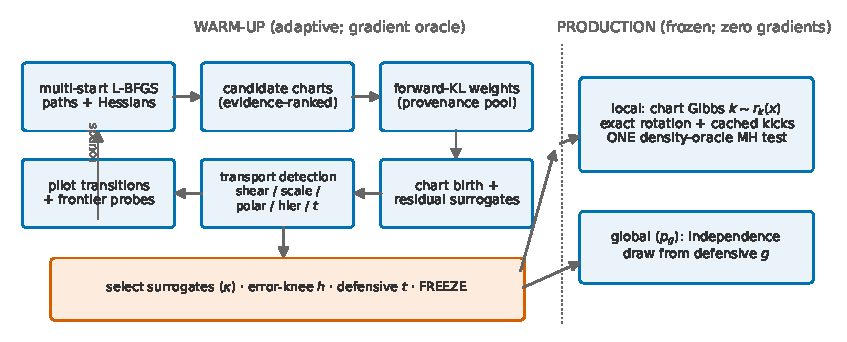
\includegraphics[width=\textwidth]{warmup_flow.pdf}
\caption{\textbf{Warm-up and production at a glance.} Warm-up (left of
the dashed line) iterates pilot sampling, transport detection, chart
birth, and weight refits, then selects surrogates, tunes the step size at
the error knee, fits the defensive component, and freezes. Production
(right) alternates the chart-conditional harmonic transition---one
target-density call---with the global independence branch.}
\label{fig:flow}
\end{figure}

\subsection{Candidate charts and evidence scores}
Multi-start L-BFGS paths supply candidate centers $\mu$; covariances are
clipped inverse Hessians
\begin{equation}
\Sigma=V\operatorname{diag}\bigl(\max(\lvert\lambda_i\rvert,
\lambda_{\min})\bigr)^{-1}V^\top,\qquad H=V\Lambda V^\top,
\label{eq:clip}
\end{equation}
ranked by the Monte Carlo evidence bound
\begin{equation}
\mathcal E_k=\frac1S\sum_{s=1}^S\bigl[-U(\mu_k+L_kz_s)\bigr]
+\frac12\log\lvert\Sigma_k\rvert,\qquad z_s\sim\mathcal N(0,I),
\label{eq:elbo}
\end{equation}
and deduplicated by Mahalanobis distance under retained charts.

\subsection{Mixture weights: forward KL on a provenance pool}
Weights maximize the concave pooled objective
\begin{equation}
w^\star=\arg\max_{w\in\Delta_{K-1}}
\sum_i\bar\omega_i\log\Bigl(\sum_kw_kq_k(x_i)\Bigr)
\label{eq:fkl}
\end{equation}
via the EM fixed point $w_k\leftarrow\sum_i\bar\omega_i\,r_k^w(x_i)$,
where the pool weights are truncated self-normalized importance ratios
\citep{ionides2008}
\begin{equation}
\bar\omega_i\;\propto\;
\min\Bigl\{\frac{\tilde\pi(x_i)}{m(x_i)},\;
\sqrt N\cdot\overline{\,\tilde\pi/m\,}\Bigr\},
\label{eq:trunc}
\end{equation}
computed against the pool's \emph{generating} mixture $m$: the balanced
mixture of every component that ever contributed pool samples, including
since-pruned ones. Substituting the current mixture for $m$ is a
proposal mismatch that we observed to collapse the fit (importance ESS
$\to1$) and delete correct charts; \eqref{eq:trunc} is a
correctness-of-fit detail, not a tuning choice.

\subsection{Surrogate selection}
Per chart, candidate force models are compared on held-out anchors by the
normalized force error
\begin{equation}
\kappa=\frac{\sum_{i\in\mathrm{val}}
\lVert f_i-\hat f(z_i)\rVert^2}
{\sum_{i\in\mathrm{val}}\lVert f_i\rVert^2},
\label{eq:kappa}
\end{equation}
whose denominator is the zero-force baseline: a model is deployed only if
$\kappa<1-\varepsilon$, with a cost-aware tie-break toward \eqref{eq:rbf}.
This rule lets a chart switch its cache \emph{off} on geometry it cannot
represent rather than degrade below exact harmonic motion.

\subsection{Residual-guided chart birth}
With coverage deficit $a(x)=\log\tilde\pi(x)-\log q(x)$, frontier states
maximize
\begin{equation}
F(x)=\bigl(a(x)-\operatorname{med}a\bigr)_+
\bigl(1-\mathrm{trust}(x)\bigr)
\label{eq:birth}
\end{equation}
over pilot states and overdispersed chart probes; promising probes are
refined by a capped ($\le4$-step) descent---enough to relax the
off-manifold error of tangent probes on curved ridges, while an uncapped
descent collapses candidates back to the dominant mode. Newborn charts
take clipped-Hessian covariances \eqref{eq:clip} with a
geometry-uncertainty widening, and weights are refit by \eqref{eq:fkl}.

\subsection{Transport detection}
\paragraph{Composed shears.} For a driver--target pair $(d,t)$, let
$\tilde q$ be the component of $(x_d-\bar x_d)^2$ orthogonal to
$\operatorname{span}\{1,x_d\}$ over the fit set. The pair is admitted
when the partial coefficient of determination
\begin{equation}
R^2_{d\to t}
=\frac{\langle\tilde q,\,x_t\rangle^2}
{\lVert\tilde q\rVert^2\operatorname{Var}(x_t)}
\label{eq:partialr2}
\end{equation}
exceeds a threshold;
$\gamma=\langle\tilde q,x_t\rangle/\lVert\tilde q\rVert^2$, the fitted
shear is peeled from the data, and the scan repeats. Plain $R^2$ is
deflated by the linear leakage of $(x_d-\bar x_d)^2$ under skewed data;
\eqref{eq:partialr2} is the skew-robust statistic.
\paragraph{Conditional scale.} For driver $v$, slopes follow from the
bias-corrected log-square regression
\begin{equation}
\log(x_i-\mu_i)^2\;\approx\;\alpha_i+\beta_i(v-\bar v)+\E\log\chi_1^2,
\qquad \E\log\chi_1^2\approx-1.2704.
\label{eq:scalereg}
\end{equation}
\paragraph{Polar.} Circle candidates come from the data mean, the
K\r{a}sa linear system \citep{kasa1976}
\begin{equation}
\begin{bmatrix}2x&2y&1\end{bmatrix}
\begin{bmatrix}c_1\\ c_2\\ t\end{bmatrix}=x^2+y^2,
\label{eq:kasa}
\end{equation}
and variance-of-radius descent from each; a candidate survives only under
density-free \emph{angular-support} gates (sector occupancy $\ge10/24$;
maximal angular gap $\le\pi$), which reject the tangent-circle
degeneracy of short-arc fits, plus a held-out density comparison against
a Gaussian alternative.
\paragraph{Hierarchical location--scale.} A (driver, location) pair scan
applies \eqref{eq:scalereg} to deviations $x_j-x_{\mathrm{loc}}$; the
shared exponent is $\gamma=\bar\beta/2$.
\paragraph{Heavy tails.} Along latent rays $z=ru$ of the dominant chart,
\begin{equation}
\rho=\frac{U(T(r_3u))-U(T(r_2u))}{U(T(r_2u))-U(T(r_1u))},
\qquad(r_1,r_2,r_3)=(3,9,27),
\label{eq:ray}
\end{equation}
equals $(r_3^2-r_2^2)/(r_2^2-r_1^2)=9$ for Gaussian tails and is $O(1)$
for polynomial tails; a measured $\rho<4$ triggers $t$-conversion with
$\nu$ matched to $\rho$. Ray probes are chain-independent, avoiding the
circularity of estimating tail weight from a chain confined to the bulk.

\subsection{Step size: dual averaging and the error knee}
Dual averaging \citep{hoffman2014} targets endpoint acceptance; a final
refinement fits the two-term error model of
Proposition~\ref{prop:accept} from matched trajectory batches at $h$ and
$h/2$:
\begin{equation}
\widehat V_{\mathrm{sur}}=\frac{16V(h/2)-V(h)}{15},
\qquad
\widehat{ch^4}=\frac{16}{15}\bigl(V(h)-V(h/2)\bigr),
\label{eq:knee}
\end{equation}
with $V(h)=\operatorname{Var}(\Delta H)$, moving $h$ to the knee
$ch^4\approx V_{\mathrm{sur}}$: below it, smaller steps buy no
acceptance because surrogate error is $h$-independent.

\begin{algorithm}[t]
\caption{Warm-up (all adaptation frozen before production)}
\label{alg:warm}
\begin{algorithmic}[1]
\State multi-start L-BFGS; Hessian charts at evidence-selected path
  points \eqref{eq:clip}--\eqref{eq:elbo}; collect
  $(x,U,\nabla U)$ anchors
\State fit weights \eqref{eq:fkl}--\eqref{eq:trunc}; prune by
  leave-one-out coverage
\State bootstrap transports from path anchors; $t$-conversion by
  \eqref{eq:ray}
\For{round $=1,\dots,B$}
  \State pilot transitions (states, anchors, frontier candidates)
  \State retry transport detection on all geometry points; birth charts
    by \eqref{eq:birth}; refit weights; rebuild caches
\EndFor
\State select surrogates by \eqref{eq:kappa}; dual-average $h$;
  error-knee refinement \eqref{eq:knee}; fit defensive component of
  \eqref{eq:defensive}; \textbf{freeze}
\end{algorithmic}
\end{algorithm}

\section{Theoretical Analysis}\label{sec:theory}
\subsection{Acceptance bounds}
\begin{proposition}[Error decomposition]\label{prop:accept}
Let $e_k(z)=\nabla_zR(T_kz)-\hat f_k(z)$ and suppose
$\lVert e_k\rVert\le\delta$ along a trajectory of total time $T$ with
$\mathcal L_p=\int_0^T\lVert p_t\rVert\,\dd t$, with $R\circ T_k$ and
$\hat f_k$ of class $C^2$ on its neighborhood. Then
\begin{equation}
\lvert\Delta H_k\rvert\;\le\;\delta\,\mathcal L_p+C_Th^2,
\qquad
\alpha_{\mathrm{loc}}\;\ge\;e^{-\delta\mathcal L_p-C_Th^2}.
\label{eq:accbound}
\end{equation}
If moreover $\hat f_k=\nabla\widehat R_k$ with
$\sup\lvert R\circ T_k-\widehat R_k-c\rvert\le\eta$, then
$\lvert\Delta H_k\rvert\le2\eta+C_Th^2$.
\end{proposition}
\begin{proof}
Along the continuous surrogate flow $\dot H_k=p^\top e_k(z)$, giving the
first term by Cauchy--Schwarz; the $O(h^2)$ term follows, for conservative $\hat f_k$, from the
backward-error bound for symmetric splittings of the surrogate
Hamiltonian \citep{leimkuhler2004}, and for non-conservative fields
from the global $O(h^2)$ trajectory-error bound of the second-order
splitting over the fixed horizon $T$. For the scalar case write
$H_k=\widehat H_k+(R\circ T_k-\widehat R_k)$; the splitting nearly
conserves $\widehat H_k$ and the difference is bounded by $2\eta$
end-to-end.
\end{proof}

\subsection{Dimension-independent target-oracle efficiency}
\begin{theorem}[Target-oracle dimension independence]\label{thm:dimfree}
Suppose that after an atlas chart, $\pi=\pi_s\otimes\mathcal N(0,I_{d-s})$
with $q$ matching the Gaussian factor exactly, charts acting
block-diagonally, and cached forces supported on the first $s$
coordinates (as induced by the active-subspace construction). Then
$\Delta H_k$ is a function of the $s$-block alone, so acceptance, the
tuned $(h,T)$, and the number of \emph{target-oracle} calls per effective
sample of $s$-block statistics are independent of $d$.
\end{theorem}
\begin{proof}
On the Gaussian block $R$ is constant and $\hat f_k$ vanishes, so the
dynamics there are the exact rotation \eqref{eq:rot}: energy is conserved
exactly, coordinate-wise, and the block contributes zero to $\Delta H_k$
deterministically. All acceptance statistics coincide with those of the
$s$-dimensional sampler, and each transition makes one density-oracle
call regardless of $d$.
\end{proof}

\begin{remark}[What is, and is not, dimension-independent]
Theorem~\ref{thm:dimfree} concerns \emph{target-oracle} efficiency.
Per-transition \emph{arithmetic} includes $O(Kd^2)$ mixture algebra
(Table~\ref{tab:cost}), and the cost of a single target evaluation may
itself grow with $d$; neither is claimed independent of dimension. In
the oracle-dominated regimes this paper targets, the oracle count is the
relevant complexity; wall-clock results (Section~\ref{sec:native})
quantify the arithmetic explicitly.
\end{remark}

\begin{corollary}[Conditioning]\label{cor:kappa}
For Gaussian targets with arbitrary covariance, an exact Laplace chart
gives $R\equiv\mathrm{const}$, acceptance one, and $O(1)$ target-oracle
units per (near-independent) effective sample, independent of $\kappa$;
the $\Theta(\sqrt\kappa)$ dependence is confined to the one-time L-BFGS
warm-up.
\end{corollary}

\subsection{Three complexity separations}\label{sec:separations}
The preceding results combine into the paper's central theoretical
statement: along the three axes on which gradient-based samplers are
known to degrade, the \emph{production} cost of PMR-HMC does not degrade
at all---the entire dependence is confined to the one-time warm-up.

\begin{theorem}[Complexity separations]\label{thm:sep}
Every production transition makes exactly one target-density-oracle call
and zero gradient-oracle calls. Moreover:
\begin{enumerate}
\item[(i)] \textbf{Conditioning.} For a Gaussian target with condition
  number $\kappa$ and an exact Laplace chart, trajectories at $T=\pi/2$
  are accepted with probability one and successive states are
  independent draws from $\pi$: $O(1)$ target-oracle units per effective
  sample, uniformly in $\kappa$. Leapfrog-based HMC requires
  $\Theta(\sqrt\kappa)$ gradient calls per effective sample
  \citep{neal2011,langmore2019}.
\item[(ii)] \textbf{Dimension.} Under the hypotheses of
  Theorem~\ref{thm:dimfree}, target-oracle units per effective sample of
  the $s$-block statistics are independent of the ambient dimension $d$.
  Optimal scaling for leapfrog HMC on product targets forces step size
  $h=\Theta(d^{-1/4})$ and hence $\Theta(d^{1/4})$ gradient calls per
  effective sample \citep{beskos2013}.
\item[(iii)] \textbf{Multimodality.} Under the tail-dominance hypothesis
  of Theorem~\ref{thm:ue}, for any measurable set $A$ the expected
  number of transitions to first entry of $A$ is at most
  $M/(p_g\,\pi(A))$, \emph{independent of the separation between modes};
  local-flow samplers have mixing times exponential in barrier height
  \citep{mangoubi2018}.
\end{enumerate}
\end{theorem}
\begin{proof}
The per-transition oracle count is Algorithm~\ref{alg:prod}. (i) With an
exact chart, $R\equiv\mathrm{const}$, so $\Delta H_k=0$ deterministically
and every proposal is accepted; at $T=\pi/2$ the rotation
\eqref{eq:rot} maps $(z,p)\mapsto(p,-z)$, and since $p$ is refreshed
i.i.d.\ $\mathcal N(0,I)$ each transition, successive positions are
independent draws from the latent Gaussian, hence from $\pi$
(Lemma~\ref{lem:aug}). (ii) is Theorem~\ref{thm:dimfree}. (iii) By the
minorization in the proof of Theorem~\ref{thm:ue},
$P(x,A)\ge(p_g/M)\,\pi(A)$ for every $x$, so the first-entry time of $A$
is stochastically dominated by a geometric random variable with success
probability $(p_g/M)\,\pi(A)$, giving the stated expectation bound. No
quantity in the bound depends on the location or separation of the
regions carrying $\pi$'s mass.
\end{proof}

\begin{remark}[Idealization and its empirical gap]
All three statements are exact-atlas idealizations; with \emph{learned}
atlases the experiments measure their realization directly (medians over
8 seeds): production cost $1.26$--$1.35$ units/ESS across
$\kappa=10^2..10^5$ (slope $0.00$ against the $\sqrt\kappa$
reference), a $24$--$37$ units/ESS plateau across $d=50..200$, and a
mode-switch rate flat in separation while NUTS's median falls to zero
(Figure~\ref{fig:scaling}). The warm-up, not production,
absorbs the $\Theta(\sqrt\kappa)$ optimization cost and the
mode-discovery problem; Section~\ref{sec:lim} discusses when warm-up
itself fails.
\end{remark}

\subsection{Cost model and amortization}\label{sec:cost}
Table~\ref{tab:cost} itemizes each phase. Writing $G$ for total warm-up
gradient calls and $N$ for production draws, per-draw target-oracle
costs compare as
\begin{equation}
\underbrace{\,c_gG/N+1\,}_{\text{PMR-HMC, amortized}}
\qquad\text{vs.}\qquad
\underbrace{\,c_gL_N\,}_{\text{NUTS}},
\label{eq:amort}
\end{equation}
with break-even draw count
\begin{equation}
N^\star\;\approx\;\frac{c_gG}{c_gL_N-1},
\label{eq:breakeven}
\end{equation}
a few hundred draws in every experiment below. $G$ is paid once per
posterior while $L_N$ is paid per draw indefinitely; chains share one
frozen atlas, dividing $G$ further.

\begin{table}[t]
\caption{Oracle and arithmetic cost by phase ($n_H$ Hessians; $A$
anchors; $L$ integrator steps; $M$ radial-basis centers; $s$ active
dimension).}
\label{tab:cost}
\centering\small
\begin{tabular}{lll}
\toprule
phase & target-oracle cost & arithmetic\\
\midrule
L-BFGS starts & $c_g\cdot$iters & $O(d)$/iter\\
Hessian charts & $c_g\,n_Hd$ & $O(d^3)$/chart\\
anchors, probes, pools & $c_gA+O(A)$ & $O(Ad^2)$\\
weight fit \eqref{eq:fkl} & --- & $O(KN_{\mathrm{pool}}d^2)$\\
surrogate fits & --- & $O(AMs+Ms^3)$\\
tuning and knee \eqref{eq:knee} & $O(10^3)$ density & ---\\
\midrule
production, local & $1$ density & $O(Kd^2+LMs)$\\
production, global & $1$ density & $O(Kd^2)$\\
NUTS, per draw & $c_gL_N$ & $O(L_Nd)$\\
\bottomrule
\end{tabular}
\end{table}

\subsection{Oracle accounting and sensitivity}\label{sec:oracleacct}
All summary efficiencies use $c_g=2.5$; raw density and gradient counts
are released with the artifacts. Because production uses zero gradient
calls, the PMR-HMC-to-NUTS efficiency ratio is monotone in $c_g$: with
per-draw costs \eqref{eq:amort} it scales as
\begin{equation}
\mathrm{ratio}(c_g)=\frac{c_gL_N}{c_gG/N+1},
\label{eq:cgsens}
\end{equation}
so moving $c_g$ from $2.5$ to $1$ multiplies reported ratios by a factor
in $[0.4,1]$ and to $4$ by a factor in $[1,1.6]$. On the
ill-conditioned Gaussian, recomputed from the 8-seed sweep with the
warm-up's density/gradient mix bounded both ways, the amortized
$\kappa{=}10^4$ ratio lies in roughly $[143,223]\times$ at $c_g{=}1$
and $[264,358]\times$ at $c_g{=}4$, around the reported $251\times$ at
$c_g{=}2.5$. No qualitative conclusion in
Section~\ref{sec:experiments} changes over $c_g\in[1,4]$.

\section{Experiments}\label{sec:experiments}
\begin{figure}[t]
\centering
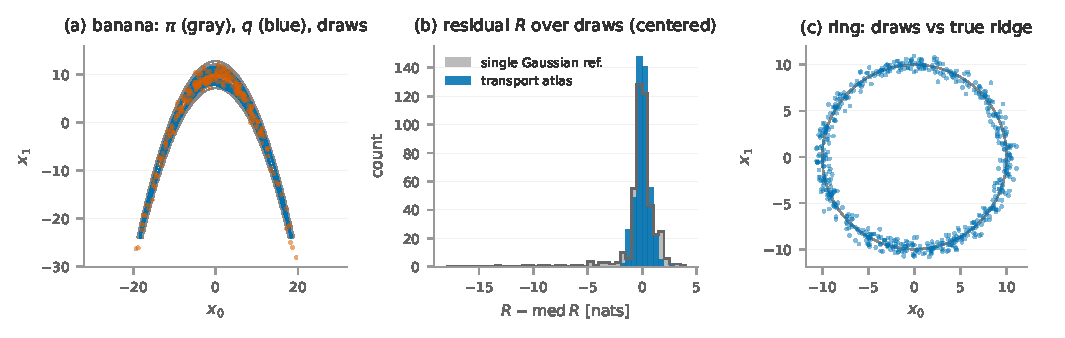
\includegraphics[width=\textwidth]{mechanics.pdf}
\caption{Mechanics. (a) The learned atlas (blue: contours of $q$ with a
fitted shear chart) reproduces the banana target (gray); production
draws (vermillion) cover both arms. (b) The core of the construction:
the residual $R=U+\log q$ under the transport atlas (blue) versus under
a moment-matched single Gaussian (gray)---the atlas flattens $R$ from a
$\sim$22-nat range to a few nats, which is what zero-gradient cached
dynamics require. (c) Visual check on the ring: draws against the true
ridge; the winding chart's harmonic angle circulates the full circle.}
\label{fig:mech}
\end{figure}

\begin{figure}[t]
\centering
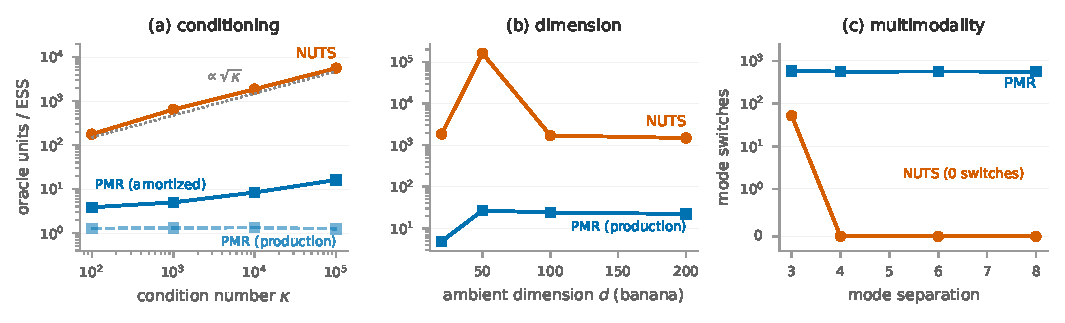
\includegraphics[width=\textwidth]{scaling.pdf}
\caption{Measured separations (target-oracle units per effective
sample; medians with interquartile bands over 8 seeds). (a) NUTS follows
the $\sqrt\kappa$ slope over $\kappa=10^2..10^5$ while PMR-HMC
production cost is flat at $1.26$--$1.35$
(Corollary~\ref{cor:kappa}); the solid blue curve includes amortized
warm-up. (b) On embedded bananas PMR-HMC production cost plateaus while
NUTS is both expensive and strongly seed-sensitive (the wide band spans
its pathological runs). (c) Mode switches versus separation: the NUTS
median falls to zero while its within-mode ESS stays high; the global
branch is flat (Theorem~\ref{thm:ue}).}
\label{fig:scaling}
\end{figure}

\begin{figure}[t]
\centering
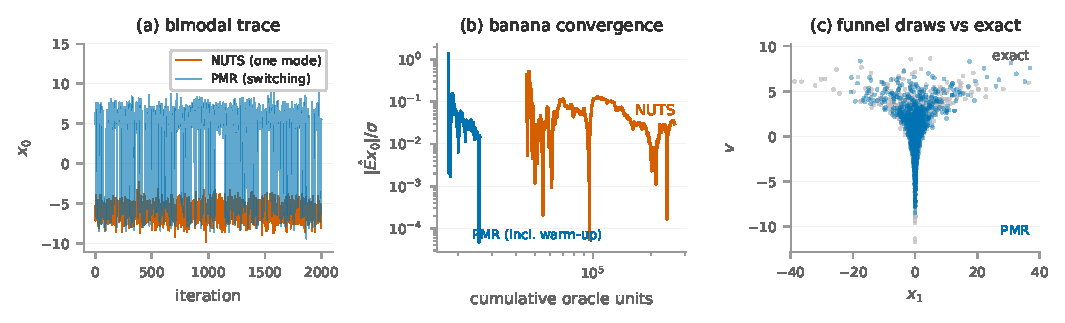
\includegraphics[width=\textwidth]{convergence.pdf}
\caption{Progression and visual checks. (a) Bimodal traces: NUTS remains
in one mode; PMR-HMC switches freely. (b) Running estimate error versus
cumulative target-oracle units on the banana (log--log): the PMR-HMC
curve is shifted by warm-up, then converges far to the left of NUTS.
(c) Funnel draws (blue) against exact samples (gray): the learned
conditional-scale chart reaches both mouth and neck.}
\label{fig:conv}
\end{figure}

\subsection{Protocol}
Every method runs on the same two final suites: the 37-posterior
posteriordb battery (gold-judged) and a curated 30-target controlled
stress panel (truth/reference-judged). The ten-method panel comprises
PMR-HMC, diagonal-mass NUTS, and dense-mass NUTS (8 seeds on
posteriordb, 4 on the stress panel), plus Pathfinder-initialized
dense-mass NUTS, ChEES-HMC, MCLMC, TESS, flow-based independence MH, a
flowMC-style flow-MALA hybrid, and NeuTra-HMC (4 seeds; the four
flow-based methods share one RealNVP architecture and training budget,
charged to their oracle counts). The three scaling sweeps use 8 seeds.
ESS is rank-normalized bulk ESS on a single chain, minimized over
coordinates; cross-seed rank-$\widehat R$ diagnostics accompany the
posteriordb battery. Accuracy is judged against analytic truth or gold
reference draws under one symmetric gate (max standardized mean error
$\le0.25\sigma$ and max log-variance error $\le0.5$); all numbers, raw
oracle counts, and scripts are released.

Per-method draw budgets and tuning, disclosed in full: PMR-HMC draws
$8{,}000$ production samples per posteriordb chain and $6{,}000$ on
the stress panel; NUTS variants $2{,}500$ after $700$--$800$ warm-up
iterations; ChEES $1{,}500$ per chain over $16$ chains after $500$
adaptation steps (identity mass, Adam $0.02$, per-chain oracle
accounting); MCLMC $8{,}000$ after the standard $2{,}000$-step
$L$/step-size auto-tune \citep{robnik2023}; the flow-based methods
$6{,}000$ ($2{,}500$ for NeuTra) after a shared $800$-step RealNVP
training run charged to their oracle counts. No covariates are
standardized for any method. Because the headline metric is
\emph{amortized} (warm-up included), a longer production chain dilutes
warm-up more for PMR-HMC than for the fast-warm-up baselines; the
scaling study reports production-only and amortized rates separately
for exactly this reason, and the crossover analysis of
Section~\ref{sec:native} quantifies the budget dependence in wall
clock.

\subsection{Complexity separations}
Figure~\ref{fig:scaling} is the measured realization of
Theorem~\ref{thm:sep}: the NUTS median grows from $153$ to $5{,}672$
units/ESS over $\kappa=10^2..10^5$ (fitted slope $0.52$) with tight
interquartile ranges, while PMR-HMC production is flat at $1.26$--$1.35$
(slope $0.00$), i.e., $365\times$ amortized and $3{,}500\times$
production-to-production at $\kappa=10^5$. Embedded bananas: PMR-HMC
production plateaus at $24$--$37$ units/ESS across $d=50..200$, while
NUTS medians range $1{,}013$--$3{,}547$ with interquartile ranges
reaching $2.5\times10^4$---on curved targets NUTS is not merely
expensive but strongly seed-sensitive. Mixtures: the NUTS median switch count falls $42\to1\to0\to0$ across
separations $3..8$ with median error rising to $0.65\sigma$ while it
reports high within-mode
ESS; PMR-HMC holds a median $\approx570$ switches and
$\le0.04\sigma$ error at every separation, with interquartile ranges of
a few tens of switches. Figure~\ref{fig:mech} shows the underlying
mechanics on the canonical geometries (atlas fit, residual
flattening, winding coverage), and Figure~\ref{fig:conv} the
corresponding bimodal traces, convergence-versus-oracle-cost curves,
and funnel draws.

\subsection{A 37-posterior benchmark drawn from posteriordb, against
ten methods}
\label{sec:pdb}
The posteriordb battery runs 37 ported posteriors (including the arK,
ARMA(1,1), and GARCH(1,1) time-series models with their constraint
Jacobians) against a ten-method panel judged on the database's gold
reference draws: PMR-HMC, diagonal-mass NUTS, and dense-mass NUTS at 8
seeds, plus Pathfinder-initialized dense NUTS, ChEES-HMC, MCLMC, and
four learned-transport samplers---TESS, flow-based independence MH,
a flowMC-style flow-MALA hybrid, and NeuTra-HMC, all four sharing one
RealNVP training budget---at 4 seeds. Cross-seed rank-$\widehat R$ is
computed per target. Table~\ref{tab:inclusion} is the inclusion audit
(37 of 46 gold-referenced posteriors; the remainder require ODE,
HMM-forward, or latent-GP infrastructure---no posterior was excluded on
account of results). Under the \emph{accuracy-gated} best criterion
applied symmetrically to all samplers (a row is contestable only when a
sampler's maximum gold error is below $0.25\sigma$ mean and $0.5$
log-variance; a violation is a failure for the violating sampler
regardless of its efficiency), \textbf{PMR-HMC is the gated-best method
on 34 of 37 posteriors against all nine baselines simultaneously}
(dense-mass NUTS takes 2, MCLMC takes 1). We report efficiency ratios
over rows where \emph{both} PMR-HMC and the baseline pass the gate---a
gate-failing chain's ESS is not a meaningful denominator, by the
paper's own argument---and give each baseline's gate-fail count
alongside. The median PMR-HMC advantage is $38\times$ over diagonal
NUTS ($35$ contested rows), $4.1\times$ over dense-mass NUTS ($35$;
$90$th percentile $44\times$), $4.0\times$ over Pathfinder-initialized
dense NUTS, $12\times$ over ChEES (which passes the gate on only $11$
of 37 rows), $10\times$ over MCLMC ($19$ rows), $95\times$ over NeuTra
($31$), and $11$--$45\times$ over TESS, flow-IMH, and the
flowMC-style hybrid, which pass the gate on at most $9$ of 37
posteriors each---their dominant failure mode on real posteriors is
accuracy, not speed (Section~\ref{sec:panel}). Dense mass adaptation shrinks the
margins exactly as expected---it is the strongest baseline---but flips
only two verdicts. Table~\ref{tab:pdb} shows representative rows; the
complete $37\times10$ table is Table~\ref{tab:pdbfull}
(Appendix~\ref{app:panels}). The three PMR
losses are informative and doubly flagged: the two accuracy failures
(\texttt{earn\_height}, an extreme heteroscedastic raw-scale tail, and
\texttt{kilpisjarvi}) are precisely the two targets whose cross-seed
rank-$\widehat R$ exceeds $1.05$ ($1.11$ and $1.26$; all other targets
$\le1.01$), corroborating the gold-error verdicts; the one efficiency
loss is noncentered eight-schools, where MCLMC is best
($43.6$ vs.\ $8.1$)---a model the practitioner has already
reparameterized is the gradient samplers' best case.
Figure~\ref{fig:pdb} visualizes ratios and accuracy.

\begin{table}[t]
\caption{Representative posteriordb rows, gold-judged, with the full
ten-method panel (min-ESS per $10^3$ target-oracle units;
PMR/NUTS/dNUTS medians over 8 seeds, other methods over 4; $^{*}$ fails
the accuracy gate; \textbf{bold} $=$ best among gate-passing methods.
All 37 rows: Table~\ref{tab:pdbfull}.)}
\label{tab:pdb}
\centering\footnotesize
\setlength{\tabcolsep}{1.8pt}
\begin{tabular}{lrrrrrrrrrrr}
\toprule
posterior & $d$ & PMR & NUTS & dNUTS & PF-dN & ChEES & MCLMC & TESS
 & f-IMH & flowMC & NeuTra\\
\midrule
logearn\_lhm & 4 & 206.3 & 0.2 & 23.7 & $1112\times$/$8.7\times$ & .01/.02\\
diamonds & 26 & 63.2 & 0.1 & 14.7 & $623\times$/$4.3\times$ & .04/.06\\
logearn\_ix & 5 & 193.6 & 0.4 & 3.7 & $438\times$/$52\times$ & .02/.04\\
logearn\_hm & 4 & 219.1 & 0.8 & 4.5 & $260\times$/$49\times$ & .02/.02\\
kid\_ix & 5 & 155.5 & 0.6 & 20.4 & $260\times$/$7.6\times$ & .02/.03\\
logearn & 3 & 239.0 & 1.1 & 4.1 & $214\times$/$58\times$ & .01/.02\\
log10earn & 3 & 214.5 & 1.2 & 1.9 & $178\times$/$115\times$ & .02/.02\\
kid\_iq & 3 & 228.1 & 2.8 & 25.9 & $81\times$/$8.8\times$ & .02/.02\\
kid\_hs & 3 & 84.4 & 9.6 & 37.6 & $8.7\times$/$2.2\times$ & .03/.04\\
kilpis & 3 & 0.6 & 0.1 & 0.2 & (fail)$^\ddagger$ & .44/.86\\
gauss\_mix & 5 & 198.9 & 37.5 & 44.2 & $5.3\times$/$4.5\times$ & .03/.04\\
gp\_regr & 3 & 226.7 & 45.0 & 43.6 & $5.0\times$/$5.2\times$ & .03/.04\\
earn\_h & 3 & 0.8 & 1.1 & 14.5 & (fail)$^\ddagger$ & .17/.90\\
es\_nc & 10 & 8.1 & 16.8 & 15.9 & $0.5\times$/$0.5\times$ & .06/.11\\
\bottomrule

\end{tabular}
\end{table}

\begin{table}[t]
\caption{posteriordb inclusion audit (46 gold-referenced posteriors, 37
ported; no posterior was excluded on account of results).}
\label{tab:inclusion}
\centering\small
\begin{tabular}{lcl}
\toprule
family & ported & reason if excluded\\
\midrule
earnings regressions (7) & 6/7 & 1 redundant standardized variant\\
kidiq (4) & 4/4 & ---\\
kidiq\_with\_mom\_work (4) & 4/4 & ---\\
mesquite forms (6) & 5/6 & 1 redundant un-logged variant\\
nes 1972--2000 (8) & 8/8 & ---\\
blr (sblri, sblrc) (2) & 2/2 & ---\\
eight\_schools NC (1) & 1/1 & ---\\
gauss mixture (1) & 1/1 & ---\\
GP (gp\_regr, gp\_pois, accel\_gp) (3) & 1/3 & latent-GP infrastructure\\
diamonds, kilpisjarvi (2) & 2/2 & ---\\
time series (arK, arma, garch) (3) & 3/3 & ---\\
HMM family (3) & 0/3 & forward-algorithm port\\
ODE (lotka--volterra, one\_comp) (2) & 0/2 & ODE-solver port\\
\midrule
total & 37/46 & \\
\bottomrule
\end{tabular}
\end{table}

\begin{figure}[t]
\centering
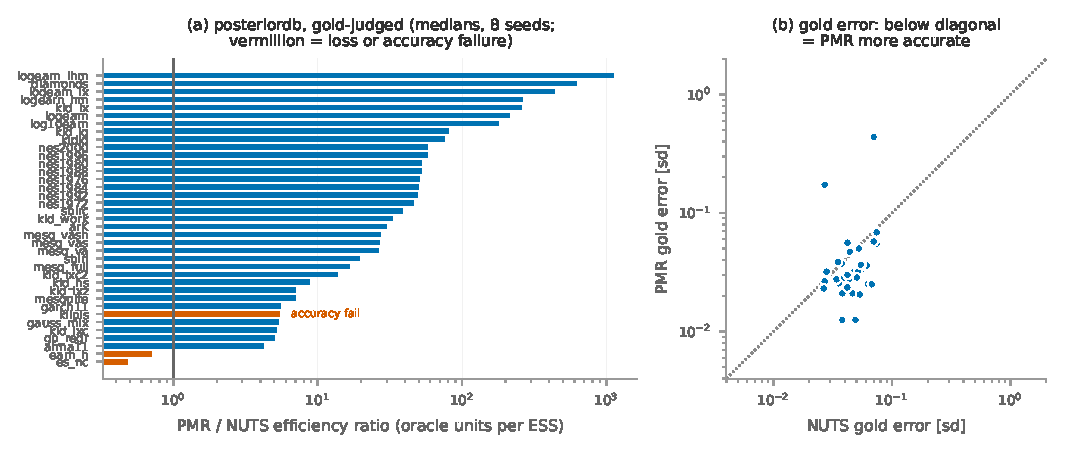
\includegraphics[width=.8\textwidth]{pdb.pdf}
\caption{posteriordb summary. (a) Efficiency ratio per posterior (log
scale). (b) Accuracy versus gold draws: points below the diagonal are
posteriors where PMR-HMC is more accurate than NUTS.}
\label{fig:pdb}
\end{figure}

\subsection{The ten-method panel: gradient samplers and learned
transports}\label{sec:panel}
Table~\ref{tab:panelsum} summarizes the panel across both suites; the
complete per-target tables are Appendix~\ref{app:panels}. Three
findings organize the comparison. \emph{First}, dense-mass NUTS is the
strongest baseline overall: it improves diagonal NUTS by an order of
magnitude on correlated targets, never fails the gate on posteriordb,
and is the runner-up by median efficiency ratio on both suites (by
gated-best count the mega-30 runner-up is MCLMC), yet PMR-HMC retains
a $4.1\times$ ($2.1\times$) both-pass median advantage on posteriordb
(mega-30), and Pathfinder initialization changes its totals only
marginally. \emph{Second}, MCLMC is the strongest baseline on
\emph{smooth, unimodal, well-scaled} targets: on the controlled mega-30
families it is gated-best on 9 of 30 rows (GLM-type regressions,
log-cosh, moderate skew---including rows where PMR's chart classes are
open problems, e.g., horseshoe and extreme skew). On the real
posteriordb suite it takes 1 of 37 rows and fails the gate on 18,
mostly low-dimensional raw-scale regressions. We flag the
interpretation honestly: MCLMC's unadjusted dynamics carry an
asymptotic bias that is a \emph{tunable} trade-off
\citep{robnik2023}, and its posteriordb gate failures conflate that
intrinsic trade-off with our tuning choices (auto-tuned $L$ and step
size, no covariate standardization; per-baseline settings are listed
in the protocol)---the safe conclusion is not that MCLMC cannot
sample these posteriors but that an aggressively tuned configuration
which excels on controlled families did not transfer, while PMR-HMC's
single configuration did. \emph{Third}, the four flow-based
methods---TESS, flow-IMH, the flowMC-style hybrid, and the
flow-preconditioned NeuTra, trained at the same budget our atlas
warm-up spends---are not competitive on real posteriors: their
dominant failure mode is accuracy (gate failures on $28$--$34$ of 37
rows for the three independence-flow samplers), and on gate-passing
rows PMR-HMC's median advantage is still $11$--$95\times$; among
gate-passing rates none exceeds dense NUTS on that suite. A single
global flow must represent the entire posterior geometry at once; the
atlas replaces that hard learning problem with several easy chart fits
plus an exact mixture, and the decomposition ablations below
(Table~\ref{tab:decomp}) locate the gain: the atlas with exact
harmonic dynamics carries most of it, the independence branch is
decisive for multimodality, and neither branch alone is correct
everywhere. On the multimodal mega-30 rows,
all nine baselines fail the accuracy gate on every mixture target
(mode-stuck: high ESS on the wrong distribution); PMR-HMC is the only
method that passes.

\begin{table}[t]
\caption{Ten-method panel summary. Row 1--2: accuracy-gated best counts
per suite (ties to the higher rate). Row 3--4: median PMR-HMC
efficiency ratio over rows where \emph{both} PMR-HMC and that baseline
pass the gate (contested-row count in parentheses)---a gate-failing
chain's ESS is not used as a denominator. Row 5--6: rows on which the
baseline fails the gate. posteriordb: 37 posteriors, gold-judged;
mega-30: 30 controlled targets, truth/reference-judged; 6 mega-30 rows
(both funnels, the $d{=}60$ hierarchical Gaussian, Rosenbrock, banana
at extreme bend, $\nu{=}2.5$ Student-$t$) have no gate-passing method.}
\label{tab:panelsum}
\centering\scriptsize
\setlength{\tabcolsep}{2.6pt}
\begin{tabular}{lrrrrrrrrrr}
\toprule
 & PMR & NUTS & dNUTS & PF-dN & ChEES & MCLMC & TESS & f-IMH & flowMC & NeuTra\\
\midrule
best (pdb) & \textbf{34} & 0 & 2 & 0 & 0 & 1 & 0 & 0 & 0 & 0\\
best (mega) & \textbf{12} & 1 & 1 & 0 & 0 & 9 & 1 & 0 & 0 & 0\\
ratio (pdb) & --- & $38\times$\,(35) & $4.1\times$\,(35) & $4.0\times$\,(35)
 & $12\times$\,(11) & $10\times$\,(19) & $29\times$\,(9) & $11\times$\,(7)
 & $45\times$\,(3) & $95\times$\,(31)\\
ratio (mega) & --- & $4.4\times$\,(16) & $2.1\times$\,(17) & $2.2\times$\,(17)
 & $3.3\times$\,(8) & $1.2\times$\,(15) & $9.3\times$\,(9) & $23\times$\,(8)
 & $38\times$\,(7) & $6.1\times$\,(15)\\
gate fails (pdb) & 2 & 0 & 0 & 0 & 26 & 18 & 28 & 30 & 34 & 6\\
gate fails (mega) & 9 & 11 & 11 & 11 & 21 & 13 & 20 & 22 & 22 & 13\\
\bottomrule
\end{tabular}
\end{table}

\subsection{Decomposition ablations: where the gain comes from}
\label{sec:ablation}
Three reduced kernels isolate the contributions, each run over 8 seeds
with the accuracy gate applied: \emph{zero-force} (atlas and exact
harmonic dynamics, surrogate forced to zero), \emph{global-only}
(independence Metropolis--Hastings from the learned $q$ alone,
$p_g{=}1$), and the full kernel. Table~\ref{tab:decomp} shows the
pattern. On atlas-explained targets the independence branch with a
strong $q$ alone is fastest (mixture2: $497$); off them it fails the
gate outright (ring: $0.4$ with $0.56\sigma$ error; banana:
$1.5$ log-variance error)---the local branch is what makes the kernel
correct beyond the atlas's explanatory reach. The atlas plus exact
harmonic dynamics carry most of the local gain: zero-force is within
$1.4\times$ of the full kernel on every target and ahead on two, with
the cached surrogate contributing its clearest factor on the ring
($45\to64$). The funnel row fails the variance gate for \emph{every}
kernel variant at this budget (as it does for all ten panel methods on
the stress suite), and is reported for completeness, not claimed as a
win. The nine baseline columns place the ablation in context: on these
four canonical geometries every baseline fails the gate on the banana,
the funnel, and the mixture, and the best gate-passing baseline on the
ring (MCLMC at $3.3$) sits $19\times$ below the full kernel---even the
\emph{reduced} PMR kernels outperform every baseline wherever either
passes. An earlier single-seed version of this table overstated the
surrogate's contribution; these 8-seed medians supersede it.

\begin{table}[t]
\caption{Decomposition ablations with the full baseline panel (min-ESS
per $10^3$ units; ablation columns and NUTS: medians over 8 seeds;
other baselines: 4 seeds from the same-target modern-baseline battery;
$^{*}$ fails the accuracy gate---a starred rate is not a valid win at
any magnitude; \textbf{bold} $=$ best gate-passing rate in the row).
The funnel row is gate-failed by every kernel variant \emph{and} every
baseline.}
\label{tab:decomp}
\centering\footnotesize
\setlength{\tabcolsep}{3.0pt}
\begin{tabular}{lrrrrrrrrrrrr}
\toprule
target & full & zero-f. & glob. & NUTS & dNUTS & PF-dN & ChEES & MCLMC
 & TESS & f-IMH & flowMC & NeuTra\\
\midrule
banana20 & 46.0 & \textbf{52.9} & 19.5$^{*}$ & 0.5$^{*}$ & 0.6$^{*}$ & 0.5$^{*}$ & 0.3$^{*}$ & 1.6$^{*}$ & 0.1$^{*}$ & 0.8$^{*}$ & 0.0$^{*}$ & 0.5$^{*}$\\
funnel10 & 2.3$^{*}$ & 6.8$^{*}$ & 0.6$^{*}$ & 0.1$^{*}$ & 0.1$^{*}$ & 0.0$^{*}$ & 0.2$^{*}$ & 3.8$^{*}$ & 0.2$^{*}$ & 0.2$^{*}$ & 0.2$^{*}$ & 0.2$^{*}$\\
mixture2 & 43.2 & 65.9 & \textbf{497.0} & 61.1$^{*}$ & 65.5$^{*}$ & 65.3$^{*}$ & 93.8$^{*}$ & 145.8$^{*}$ & 23.0$^{*}$ & 24.1$^{*}$ & 3.4$^{*}$ & 25.9$^{*}$\\
ring20 & \textbf{63.7} & 45.4 & 0.4$^{*}$ & 2.1 & 1.8 & 2.0 & 0.7$^{*}$ & 3.3 & 0.2$^{*}$ & 0.2$^{*}$ & 0.0$^{*}$ & 1.4\\
\bottomrule

\end{tabular}
\end{table}

\subsection{A deployed decision model at scale}\label{sec:vilya}
On a faithful reproduction of a production two-stage control-function
hurdle negative-binomial advertising model, seed-replicated over 4
seeds: median $21\times$ at $C{=}8$ campaigns ($d{=}37$) and
$11\times$ at $C{=}50$ ($d{=}163$), with substantial seed variance at
the larger size (per-seed rates $0.21$--$3.09$ ESS per $10^3$
units)---an earlier single-seed run showing $190\times$ at $C{=}50$
was a favorable draw and is superseded by these medians. Both samplers
degrade with $C$; in fact PMR-HMC's own median rate falls
\emph{more} ($9.3\times$, driven by two poor warm-up seeds, versus
$4.7\times$ for NUTS), while remaining $\approx11\times$ more
oracle-efficient at $C{=}50$; at $C{=}120$ ($d{=}373$) the current
warm-up budget fails to establish acceptance (Section~\ref{sec:lim}).

We additionally measured wall clock through the packaged library
(Section~\ref{sec:native}; Python-callback density, one JIT-compiled
evaluation per transition) at three campaign tiers. At $C{=}30$
($d{=}103$): warm-up $81$\,s, production $12.4$\,s per $10^3$ ESS at
acceptance $0.14$; at $C{=}60$ ($d{=}193$): $258$\,s and $47.6$; at
the largest tier $C{=}120$ ($d{=}373$) warm-up fails to establish
acceptance ($0.02$), confirming the ceiling. Fully JIT-compiled NUTS
on the same port is faster in wall clock at every tier
($3.8/10.1/24.1$\,s per $10^3$ ESS). At $C{=}30$ and $C{=}60$ the two
samplers' first moments agree to within $0.25$ posterior standard
deviations on the recorded coordinates (both estimates carry sampling
noise at these ESS); at $C{=}120$ PMR-HMC's ESS of $13$ admits no
meaningful agreement check. The reading is the crossover analysis of
Section~\ref{sec:native} in miniature: this port's likelihood
compiles to microseconds, so gradients are effectively free and the
oracle-cost separation does not convert into wall clock. For models
of this kind the atlas kernel's wall-clock case requires an
oracle-expensive deployment or heavy re-use of one fitted atlas, and
the binding limitation at whale scale is the warm-up dimension
ceiling, whose block-structured remedy we outline in
Section~\ref{sec:lim}.

\subsection{A 30-target controlled stress panel}\label{sec:mega}
To probe the failure surface systematically under the full ten-method
panel, we curated 30 targets from an 18-family parametric library
(dimension $5..200$, condition number to $10^5$, correlation to $0.95$,
tail index $\nu=2.5..10$, curvature, mode separation, GLM size,
hierarchy depth): every family represented, several at both an easy
and a hard setting, with every \emph{known PMR failure family
deliberately retained} (funnels, hierarchical Gaussians, horseshoe,
extreme skew, Rosenbrock, shell).
Under the symmetric gate, PMR-HMC is gated-best on 12 of 30 rows,
MCLMC on 9, and on 6 rows \emph{no} method passes (both funnels, the
$d{=}60$ hierarchical Gaussian, Rosenbrock, banana at extreme bend,
and $\nu{=}2.5$ Student-$t$, where the variance gate is brutal for
every sampler). The structure is informative. PMR-HMC's wins
concentrate exactly where Theorem~\ref{thm:sep} operates: all three
mixture rows (it is the \emph{only} gate-passing method on any
multimodal target), all correlated/ill-conditioned Gaussians
(e.g.\ $\rho{=}0.95$: $191.0$ vs.\ dense-NUTS $34.1$; $\kappa{=}10^5$:
$80.9$ vs.\ $22.3$), the easy banana and the ring (the hard banana is
a no-pass row; the squiggle is a dead-heat tie awarded to TESS by
rounding), and the diabetes and Poisson regressions. Its losses are
the documented open chart-class problems---horseshoe and extreme skew
($\alpha{=}6$) fail the gate outright, and on smooth
exponential-tailed or GLM-type rows (log-cosh, logistic, probit,
negative-binomial, Cauchy-noise, hierarchical binomial) MCLMC's tuned
dynamics are $1.1$--$6.6\times$ faster---plus one honest surprise:
dense-mass NUTS edges PMR on the small production BCF variant ($15.8$
vs.\ $9.7$ at $d{=}49$), though not at production scale
(Section~\ref{sec:vilya}). The full $30\times10$ table with per-row
gate flags is Table~\ref{tab:megafull} (Appendix~\ref{app:panels});
Section~\ref{sec:failures} tabulates every non-win row of both suites
with its diagnosed mechanism.

\subsection{Failure analysis: every row PMR-HMC does not win}
\label{sec:failures}
Across both suites there are 21 rows on which PMR-HMC is not the
gated-best method: 3 on posteriordb and 18 on mega-30. None is
mysterious; each traces to one of four mechanisms, tabulated in
Table~\ref{tab:failures} with the diagnosed root cause.

Each mechanism claim below was tested by a dedicated probe
(Figure~\ref{fig:failures}): production acceptance measured on every
failing row, the triangular-chart fitter run on warm-up-style pool
draws \emph{versus} gate-passing reference draws, and the residual
spread $\operatorname{sd}(R)$ evaluated on reference draws under the
fitted atlas. The probes corrected two of our initial hypotheses,
noted below.

\emph{(A) Representation or detection: the atlas family cannot
express, or its detector cannot find, the structure.} The shell target
loses to MCLMC ($3.6$ vs.\ $8.1$) because the polar chart unwraps a
\emph{planar} ring; a $d$-sphere shell concentrates on a norm level
set and would need a radial chart (predicted fix, not yet tested). The
extreme-bend banana ($b{=}0.2$, $d{=}30$; no method passes) is a
measured expressiveness deficit: the fitted atlas leaves
$\operatorname{sd}(R)=1.07$ nats on reference draws versus $0.52$ on
the easy banana it wins---and its acceptance is \emph{healthy}
($0.48$), the signature of a chain that moves well inside a reference
that misses curvature. The horseshoe belongs here too, which we
learned from the probe: the triangular chart's log-square driver scan
finds \emph{no} driver even when handed $3{,}000$ gate-passing
reference draws (while firing spuriously on pool draws)---a
\emph{detector} gap, not a data gap, and our initial
acquisition-only explanation was wrong.

\emph{(B) Acquisition: the chart class and detector work, but warm-up
data never exposes the structure.} The $\alpha{=}6$ skew target is the
proven case: the same fitter recovers strong skew
($\varepsilon=0.74$) from reference draws but only $\varepsilon=0.38$
from the warm-up pool, and the admitted chart is starved of
forward-KL responsibility by the co-located Gaussian components
(acceptance $0.027$). Deep hierarchies (\texttt{hgauss60}:
$15\sigma$ median error, acceptance $0.03$) fail the same way, and
the Rosenbrock valley is the purest instance: the shear fitter
recovers the correct chart when handed oracle valley data, but
warm-up exploration never collects such data (the success-history DE
explorer ablation returned null, Section~\ref{sec:negative}). The
funnels and eight-schools sit between (B) and the budget ceiling,
with degraded (not collapsed) acceptance $0.09$--$0.24$.

The acceptance probe (Figure~\ref{fig:failures}a) separates three
deployment-observable signatures, none requiring reference draws:
acquisition failures \emph{collapse} ($0.008$--$0.03$ versus
$\ge0.88$ on wins), budget-limited rows degrade ($0.09$--$0.24$), and
representation failures keep healthy acceptance while the chain
samples a subtly wrong law---the one signature that instead requires
the cross-seed rank-$\widehat R$ diagnostic, which catches both such
cases on posteriordb ($1.11$, $1.26$).

\emph{(C) No-advantage regime: the geometry is already easy for
gradient samplers.} On hand-noncentered eight-schools (posteriordb),
smooth well-scaled GLM rows (logistic, probit, negative-binomial,
Cauchy-noise, log-cosh, hierarchical binomial), and the small
production-BCF variant, PMR-HMC \emph{passes} the accuracy gate but a
tuned gradient sampler is $1.1$--$6.6\times$ faster per oracle unit:
when the posterior is close to an isotropic Gaussian after trivial
rescaling, an atlas has nothing to explain and its warm-up is pure
overhead. These are efficiency losses, not correctness failures.

\emph{(D) Reference-limited rows.} \texttt{earn\_height} (extreme
heteroscedastic raw-scale tail) and \texttt{kilpisjarvi} are genuine
atlas misfits---and both are flagged \emph{without gold draws} by
cross-seed rank-$\widehat R$ ($1.11$, $1.26$); on $\nu{=}2.5$
Student-$t$ the population variance barely exists and every method
fails the variance gate, a limit of the gate itself as much as of any
sampler.

The remedies map one-to-one: (A) a radial chart, richer shear
elements, and---for the horseshoe---a shrinkage-aware driver detector
(the inverse-KL triangular objective of Section~\ref{sec:lim}
subsumes the current scan); (B) visited-state refits and
population-based acquisition (Section~\ref{sec:lim}); (C) is
inherent---the correct reading is that PMR-HMC's advantage is a
function of how much structure the posterior has for an atlas to
remove; (D) is shared by all methods.

\begin{figure}[t]
\centering
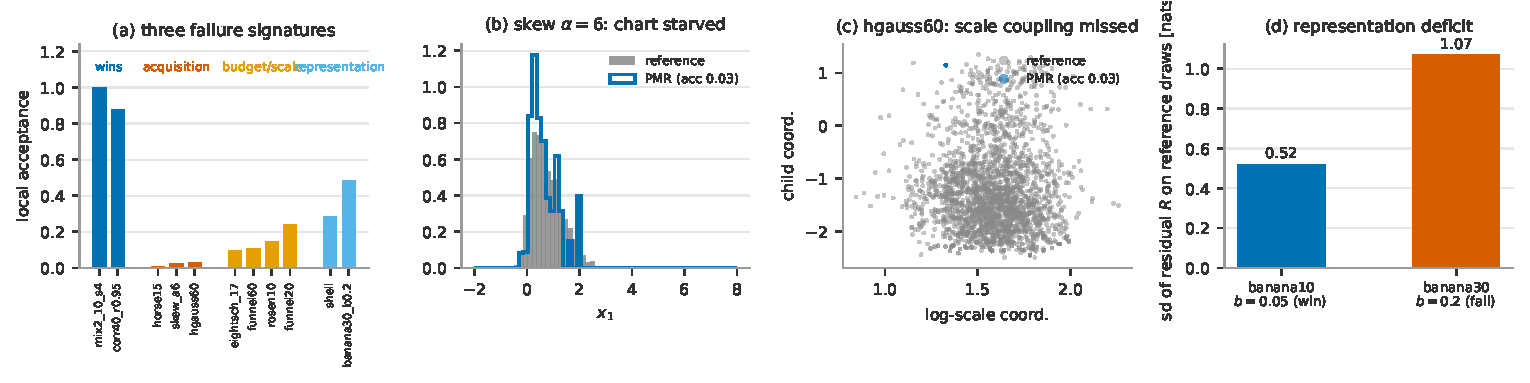
\includegraphics[width=\textwidth]{failures.pdf}
\caption{Failure-analysis probes. (a) Production acceptance separates
three failure signatures: acquisition failures collapse
($0.008$--$0.03$), budget-limited rows degrade ($0.09$--$0.24$),
representation failures keep healthy acceptance ($0.29$--$0.48$)
while sampling a subtly wrong law; wins sit at $0.88$--$1.0$.
(b) The $\alpha{=}6$ skew miss: PMR draws (blue) versus reference
(gray)---the admitted triangular chart is starved and under-corrects
the skew. (c) The $d{=}60$ hierarchical Gaussian: the chain never
tracks the scale--child coupling. (d) The extreme-bend banana's
measured expressiveness deficit: residual spread on reference draws
doubles relative to the winning easy-banana row.}
\label{fig:failures}
\end{figure}

\begin{table}[t]
\caption{Every non-win row, diagnosed; the acc.\ column is the
measured production acceptance from the verification probe. Class: A
$=$ missing chart class \emph{or} detector, B $=$ warm-up
acquisition, C $=$ no-advantage regime (gate-passing efficiency
loss), D $=$ reference-limited. ``none'' $=$ no method passes the
gate on that row.}
\label{tab:failures}
\centering\footnotesize
\setlength{\tabcolsep}{4pt}
\begin{tabular}{lllll}
\toprule
row(s) & winner & class & acc. & diagnosed cause (probe-verified)\\
\midrule
shell & MCLMC & A & .29 & polar chart is planar; radial chart is the predicted fix\\
banana $b{=}0.2$, $d{=}30$ & none & A & .48 & expressiveness: $\operatorname{sd}(R)$ $1.07$ vs $0.52$ nats on the win\\
horseshoe ($d{=}15$) & MCLMC & A & .008 & driver scan finds nothing even on reference draws\\
skew $\alpha{=}6$ & MCLMC & B & .027 & fitter recovers $\varepsilon{=}0.74$ from reference, $0.38$ from pool\\
hgauss60 & none & B & .03 & scale coupling unexposed; $15\sigma$ error\\
funnels, 8-schools & none/NUTS & B & .09--.24 & degraded at budget; between (B) and the $d$ ceiling\\
Rosenbrock $d{=}10$ & none & B & .14 & valley data never acquired (fitter itself correct)\\
GLM rows ($\times6$) & MCLMC & C & --- & near-Gaussian after rescaling; $1.1$--$6.6\times$\\
eight-schools NC (pdb) & MCLMC & C & --- & hand-noncentered; atlas has nothing to remove\\
production BCF $d{=}49$ & dNUTS & C & --- & dense mass suffices (hypothesis, not probed)\\
squiggle $f{=}4$ & TESS & C & --- & dead heat ($15.3$ vs $15.3$), tie by rounding\\
earn\_height & dNUTS & D & --- & heteroscedastic raw-scale tail; $\widehat R\,1.11$\\
kilpisjarvi & dNUTS & D & --- & all methods $\le0.6$; $\widehat R\,1.26$\\
Student-$t$ $\nu{=}2.5$ & none & D & --- & variance gate unattainable for every sampler\\
\bottomrule
\end{tabular}
\end{table}

\subsection{A production boundary study and a delayed-rejection
remedy}\label{sec:boundary}
The warm-up ceiling of Section~\ref{sec:vilya} was measured on
synthetic feature frames. To locate the boundary on real data we
ported a deployed hierarchical zero-inflated negative-binomial
advertising model---two-stage control function, per-campaign
hierarchy, Hill spend saturation---faithfully to the real feature
frame of the largest production shop in the fleet (``shop W''): 41
campaigns, $7{,}135$ rows, $d{=}618$ unconstrained parameters. The
production baseline, nutpie NUTS at $1{,}000$ tuning $+$ $1{,}500$
draws $\times$ 4 chains and target acceptance $0.95$, takes
$1{,}304$\,s of wall clock for min-ESS $365$ with zero divergences,
spending a mean $347.9$ leapfrog steps per draw at mean tree depth
$7.8$---versus $52$ steps per draw for the same model on a synthetic
frame: the real data sharpen the posterior geometry by roughly
$7\times$. Raw PMR-HMC fails completely here: local acceptance
$0.004$, the atlas collapsed to $K{=}1$, mean errors of $9\sigma$.
The failure is geometric rather than dimensional---on a $d{=}189$
synthetic version of the model the same warm-up had already failed at
acceptance $0.003$.

To identify \emph{which} structure is missing, we fitted a capacity
ladder of reference families, every rung from properly adapted
oracle-quality NUTS draws ($800$ draws, min-ESS $96$)---so warm-up
acquisition is removed from the experiment entirely---and scored each
by $\operatorname{sd}(R)$, $R=U+\log q$, on held-out draws
(Table~\ref{tab:ladder}). A block-diagonal Gaussian along the model's
per-campaign structure leaves $28.4$ nats; adding tied sinh-arcsinh
marginal warps (shapes pooled across the 41 exchangeable campaign
blocks) \emph{worsens} the held-out residual to $29.3$, so marginal
non-Gaussianity is not the obstruction; an arrow-structured
conditional Gaussian following the model's own graph (campaign blocks
conditioned on the globals) reaches $23.0$; a full shrunk covariance
$18.7$; full covariance plus tied marginal warps $16.5$. Roughly
$16$ nats of \emph{nonlinear} cross-coordinate dependence---copula
structure---remain after the marginal and every linear dependence
hypothesis have been falsified.

\begin{table}[t]
\caption{The capacity ladder on shop W ($d{=}618$). Every reference
family is fitted from oracle-quality NUTS draws ($800$ draws, min-ESS
$96$) and scored by the spread of the residual $R=U+\log q$ on
held-out draws; smaller is better, and acceptance requires order
$1$--$3$ nats in total.}
\label{tab:ladder}
\centering\small
\begin{tabular}{lr}
\toprule
reference family & $\operatorname{sd}(R)$ [nats]\\
\midrule
block-diagonal Gaussian (per-campaign $13$-dim blocks $+$ globals) & $28.4$\\
\quad$+$ tied sinh-arcsinh marginal warps (pooled shapes) & $29.3$\\
arrow-structured conditional Gaussian (blocks $\mid$ globals) & $23.0$\\
full shrunk covariance & $18.7$\\
full covariance $+$ tied marginal warps & $16.5$\\
\bottomrule
\end{tabular}
\end{table}

The number matters because of how residual spread converts to
acceptance (Proposition~\ref{prop:accept}): acceptance requires a
total residual of order $1$--$3$ nats, and residual error adds across
coordinates, so a sampler built on any single global map needs
per-coordinate fidelity of order $1/d$. The measured per-coordinate
error here is
\begin{equation}
\varepsilon_{\mathrm{coord}}
\;=\;\frac{16.5}{618}
\;=\;0.027\ \text{nats},
\qquad
d\times\varepsilon_{\mathrm{coord}}
\;\approx\;16.5\ \text{nats}
\;\gg\;\text{a few nats},
\label{eq:fidelity}
\end{equation}
excellent per coordinate and fatal in aggregate. This fidelity
law---$d$ times per-coordinate residual error must not exceed a few
nats---precisely delimits the method's competence region, and
explains with the same numbers both the posteriordb dominance at
$d\le60$ and the failure at $d{=}618$.

The remedy follows from the diagnosis: keep the one-density-call
economics where the atlas is right, and fall back to gradients
\emph{inside the same exact kernel} where it is wrong. We prototyped
a delayed-rejection hybrid \citep{green2001,modi2023}: each
transition first attempts the chart move of Algorithm~\ref{alg:prod}
at one density call; on rejection, a second stage proposes a
preconditioned leapfrog trajectory with the atlas covariance as mass
matrix, accepted with the Green--Mira two-stage ratio
\begin{equation}
\alpha_2
\;=\;1\wedge
\frac{e^{-H_2(y,p_y)}\,\bigl(1-\alpha_1^{\mathrm{ghost}}(y)\bigr)}
     {e^{-H_2(x,p_x)}\,\bigl(1-\alpha_1(x)\bigr)},
\label{eq:dr}
\end{equation}
where $H_2$ is the preconditioned Hamiltonian, $\alpha_1(x)$ the
realized stage-one acceptance probability, and
$\alpha_1^{\mathrm{ghost}}(y)$ the acceptance probability of a
freshly sampled ghost stage-one attempt launched from the stage-two
endpoint; because the stage-one auxiliaries (momentum, rotation
angle) are position-independent, sampling the ghost attempt is
legitimate and the composed kernel is exact. The stage-two step size
is dual-averaged to a target acceptance of $0.65$ ($192$ leapfrog
steps here).

We label the result as what it is---a single-seed prototype, not a
benchmark. On shop W every transition escalates (escalation rate
$1.0$: the atlas is wrong everywhere, exactly as the ladder
predicts), stage-two acceptance is $0.758$, and $3{,}000$ draws yield
min-ESS $506$ with a maximum mean gap of $0.17$ standard deviations
against the nutpie reference. Production wall clock is $328$\,s with
the gradient warm-up pilot amortized (e.g.\ reusing the previous
retrain's draws, the natural production pattern) and $824$\,s cold
including an $800$-draw pilot: $648$\,s per $10^3$ ESS warm and
$1{,}627$ cold, versus $3{,}571$ for the production nutpie
configuration---$5.5\times$ and $2.2\times$. On an easy target
(banana, $d{=}20$) with its regular multi-chart atlas, the same
kernel takes the chart move on $58\%$ of transitions and reaches
min-ESS $1{,}270$ in $3.7$\,s total.

The design point is the failure mode: the hybrid is exact everywhere,
inherits the one-density-call-per-draw economics wherever the atlas
is right, and \emph{degrades into} a preconditioned gradient sampler,
rather than failing, wherever it is wrong---rejection itself acting
as a free, oracle-free detector of atlas failure. The same rejection
signal is the natural trigger for refining the caches of
Section~\ref{sec:surrogate} online, in the spirit of the
refinement-triggered local approximations of \citet{conrad2016},
though refinement remains frozen here (Section~\ref{sec:lim}). The
insurance is not free on easy targets: the banana's $42\%$
escalations cost $\approx19$ target-oracle units per draw against
$\approx1$ for the pure kernel. Multi-seed validation, a true
dynamic-trajectory second stage, and integration into the released
library are left as engineering; the general lesson is broader than
this model---every transport-, flow-, or VI-referenced sampler obeys
the same additive fidelity law \eqref{eq:fidelity}, and delayed
rejection is the principled composition of any such reference with
gradient methods.

\subsection{Wall clock: native kernel, both regimes}\label{sec:native}
A $\sim$700-line C kernel consumes the frozen atlas (all chart classes,
both cache types, winding-branch and Gamma-auxiliary sampling) at
$0.13$--$385\,\mu$s per draw, with target-formula parity $\le10^{-12}$
against the JAX implementation on the 13-target parity study
($\le7.3\times10^{-12}$ across all 66 native-family targets) and
statistically indistinguishable acceptance. We report both wall-clock
regimes honestly, on the 66 parametric-suite targets with native C
density implementations (4 seeds, identical double precision).
\emph{Production rate}: the C kernel attains higher ESS/s than fully
JIT-compiled NUTS on 54 of 66 targets, median $13\times$, exceeding
$10^2$--$10^5\times$ on correlated, ill-conditioned, and multimodal
targets. \emph{End-to-end at a small budget}: charging PMR-HMC's Python
warm-up against a request of only $1{,}000$ effective samples, NUTS is
faster on the majority of targets (PMR-HMC wins 17 of 66)---at tiny
budgets the warm-up dominates and a JIT-compiled gradient sampler is
hard to beat on easy targets. The crossover budget---the requested ESS
beyond which PMR-HMC wins end-to-end---has median $\approx4{,}500$ ESS
(interquartile $730$--$11{,}400$) over the 54 production-faster
targets. This is precisely the amortization analysis of
Section~\ref{sec:cost} realized in wall clock: single short chains on
easy targets favor NUTS; multi-chain runs, large ESS budgets, repeated
re-use of a fitted atlas (the production setting of
Section~\ref{sec:vilya}), and any target hard enough that NUTS's
per-ESS cost blows up all sit far past the crossover.

\subsection{Calibration as an implementation audit}
Exactness follows from the invariant-kernel construction
(Section~\ref{sec:exact}); simulation-based calibration provides an
end-to-end \emph{implementation} check. Over three prior-predictive
families $\times$ 30 replications, rank statistics are uniform (worst
family: 1 of 8 parameters below $p{=}0.05$, consistent with chance at
the $5\%$ level, where $0.4$ rejections among 8 tests are expected).
Scaling
SBC to several hundred replications per family is planned for the
revision.

\subsection{Further ablations and negative results}\label{sec:negative}
A Pareto/CMA-ES environmental-selection atlas builder
\citep{hansen2001,deb2002} attains parity with the score rule while
producing leaner atlases (funnel $K{=}7$ vs.\ $11$); a success-history DE
explorer \citep{tanabe2014} for warm-up acquisition produced a null
result (2 seeds $\times$ 4 targets), recorded to delimit what does not
yet solve valley acquisition. Removing the provenance correction
\eqref{eq:trunc} collapses atlases (importance ESS $\to1$); replacing
branch sampling \eqref{eq:branch} by a principal branch measurably
breaks calibration.

\section{Limitations}\label{sec:lim}
(1) Hand-noncentered models are the gradient samplers' best case; our
margin there is small or negative (MCLMC takes noncentered
eight-schools). (2) Products of coupled funnels (horseshoe priors)
defeat the current warm-up: the triangular chart could express them,
but the pool never exhibits the per-coordinate scale variation its
driver scan needs. (3) Warm-up has a
dimension ceiling near $d\approx400$ under fixed budgets; the
boundary study of Section~\ref{sec:boundary} sharpens this from a
budget limit into a fidelity law---residual error adds across
coordinates, so any single global map needs per-coordinate error of
order $1/d$---and shows that block-structured construction alone
cannot fix it (the measured residual is dominated by nonlinear
cross-coordinate dependence); the delayed-rejection hybrid of that
section is the demonstrated remedy at $d{=}618$, so far on a single
seed. (4) Valley
data acquisition (Rosenbrock-class) is solved at the chart level but not
yet at the warm-up-exploration level. (5) The warm-up gradient bill is
$\Theta(\sqrt\kappa)$, paid once. (6) ODE, HMM, and latent-GP posterior
families await ports (Table~\ref{tab:inclusion}). (7) All guarantees
are for the frozen kernel; online atlas refinement requires a
cross-fitted ensemble construction left to future work. (8) Uniform
ergodicity is conditional on tail dominance (Theorem~\ref{thm:ue}); the
defensive component makes the condition plausible, not automatic.
(9) Strong skewness remains open at the acquisition level. The
sinh-arcsinh triangular chart of Section~\ref{sec:charts}---a
restricted Knothe--Rosenblatt form in the spirit of adaptive transport
maps \citep{marzouk2016,parno2018}---already closes the
exponential-tail gap (log-cosh now passes the gate) and helps moderate
skew, but at $\alpha{=}6$ skew and on the horseshoe the fitted chart is
starved: forward-KL responsibilities concentrate on the Gaussian
components, and the L-BFGS-anchored warm-up pool does not expose the
driver variation the fit needs. The remedies are richer triangular
elements fitted by the convex, coordinate-separable inverse-KL
objective (whose first-order conditions are Stein-type generalized
moment conditions subsuming our hand-crafted detectors), refitting
transports from visited states across warm-up rounds, and the
acquisition improvements of (4). The winding chart survives on
topology grounds.

\section{Conclusion}
Removing learned transport structure first, and approximating only the
residual, converts a broad class of practitioner posteriors into
near-independent sampling at one target-density evaluation per draw. The
construction is exact by design at every extension point---arbitrary
cached forces, winding charts, heavy-tailed charts---realizes measured
complexity separations against strong modern baselines, and compiles to
a kernel fast enough that the oracle, rather than the sampler, is again
the dominant cost of Bayesian computation.

\appendix
\section{Complete Ten-Method Panel Results}\label{app:panels}
Both tables report median min-ESS per $10^3$ target-oracle units
(density $=1$ unit, gradient $=2.5$); $^{*}$ marks an accuracy-gate
violation (max standardized mean error $>0.25\sigma$ or max
$|\log|$-variance error $>0.5$ against gold draws or analytic
truth/reference moments); \textbf{bold} marks the best rate among
gate-passing methods in the row; ``--'' marks a method that errored.
PMR/NUTS/dense-NUTS medians are over 8 seeds on posteriordb and 4 on
mega-30; all other methods over 4 seeds.

\begin{landscape}
\begin{table}
\caption{posteriordb: 37 posteriors $\times$ 10 methods, gold-judged.}
\label{tab:pdbfull}
\centering\footnotesize
\begin{tabular}{lrrrrrrrrrr}
\toprule
target & PMR & NUTS & dNUTS & PF-dN & ChEES & MCLMC & TESS & f-IMH & flowMC & NeuTra \\
\midrule
pdb\_arK & \textbf{147.0} & 4.9 & 47.3 & 47.8 & 11.9 & 9.4 & 3.9 & 3.7 & 0.1$^{*}$ & 15.3 \\
pdb\_arma11 & \textbf{170.5} & 40.2 & 43.3 & 42.2 & 21.4 & 55.1 & 1.2 & 0.0$^{*}$ & 25.2$^{*}$ & 9.6 \\
pdb\_diamonds & \textbf{63.2} & 0.1 & 14.7 & 10.1 & 0.0$^{*}$ & 0.1$^{*}$ & 0.0$^{*}$ & 0.0$^{*}$ & 0.0$^{*}$ & 0.0 \\
pdb\_earn\_h & 0.8$^{*}$ & 1.1 & \textbf{14.5} & 10.5 & 17.6$^{*}$ & 0.1$^{*}$ & 0.0$^{*}$ & 0.0$^{*}$ & 50.2$^{*}$ & 0.4$^{*}$ \\
pdb\_es\_nc & 8.1 & 16.8 & 15.9 & 18.1 & 3.5 & \textbf{43.6} & 10.6 & 11.6 & 1.8 & 14.0 \\
pdb\_garch11 & \textbf{63.6} & 11.6 & 17.7 & 17.8 & 4.7 & 24.7 & 8.9 & 6.0 & 1.4 & 9.6 \\
pdb\_gauss\_mix & \textbf{198.9} & 37.5 & 44.2 & 48.7 & 18.5 & 47.0 & 3.9 & 1.2 & 0.5$^{*}$ & 10.8 \\
pdb\_gp\_regr & \textbf{226.7} & 45.0 & 43.6 & 43.2 & 94.6 & 93.0 & 31.7 & 31.9 & 4.9 & 14.4 \\
pdb\_kid\_hs & \textbf{84.4} & 9.6 & 37.6 & 33.1 & 96.3$^{*}$ & 0.5$^{*}$ & 0.0$^{*}$ & 0.0$^{*}$ & 0.0$^{*}$ & 2.5 \\
pdb\_kid\_iq & \textbf{228.1} & 2.8 & 25.9 & 17.1 & 18.4$^{*}$ & 0.2$^{*}$ & 0.0$^{*}$ & 0.0$^{*}$ & 0.0$^{*}$ & 1.6 \\
pdb\_kid\_ix & \textbf{155.5} & 0.6 & 20.4 & 15.3 & 15.2$^{*}$ & 0.1$^{*}$ & 0.0$^{*}$ & 0.0$^{*}$ & 0.1$^{*}$ & 0.1$^{*}$ \\
pdb\_kid\_ixc & \textbf{165.6} & 32.2 & 38.8 & 36.2 & 64.0$^{*}$ & 0.3$^{*}$ & 0.0$^{*}$ & 0.0$^{*}$ & 0.0$^{*}$ & 0.6 \\
pdb\_kid\_ixc2 & \textbf{191.5} & 14.0 & 43.2 & 38.6 & 64.5$^{*}$ & 0.3$^{*}$ & 0.0$^{*}$ & 0.0$^{*}$ & 0.0$^{*}$ & 0.3 \\
pdb\_kid\_ixz & \textbf{183.1} & 25.9 & 32.0 & 25.7 & 65.6$^{*}$ & 0.3$^{*}$ & 0.0$^{*}$ & 0.0$^{*}$ & 0.1$^{*}$ & 0.0$^{*}$ \\
pdb\_kid\_work & \textbf{175.1} & 5.3 & 28.7 & 23.9 & 90.7$^{*}$ & 0.3$^{*}$ & 0.0$^{*}$ & 0.0$^{*}$ & 0.0$^{*}$ & 0.1$^{*}$ \\
pdb\_kidiq & \textbf{199.1} & 2.6 & 19.4 & 12.5 & 0.0$^{*}$ & 0.1$^{*}$ & 0.0$^{*}$ & 0.0$^{*}$ & 0.0$^{*}$ & 0.5 \\
pdb\_kilpis & 0.6$^{*}$ & 0.1 & \textbf{0.2} & 0.2 & 33.0$^{*}$ & 0.1$^{*}$ & 0.0$^{*}$ & 0.0$^{*}$ & 0.0$^{*}$ & 0.0$^{*}$ \\
pdb\_log10earn & \textbf{214.5} & 1.2 & 1.9 & 1.4 & 23.1$^{*}$ & 0.1$^{*}$ & 0.0$^{*}$ & 0.0$^{*}$ & 0.0$^{*}$ & 1.3 \\
pdb\_logearn & \textbf{239.0} & 1.1 & 4.1 & 2.6 & 19.2$^{*}$ & 0.1$^{*}$ & 0.0$^{*}$ & 0.0$^{*}$ & 50.1$^{*}$ & 0.8 \\
pdb\_logearn\_hm & \textbf{219.1} & 0.8 & 4.5 & 3.2 & 12.7$^{*}$ & 0.1$^{*}$ & 0.0$^{*}$ & 0.0$^{*}$ & 0.0$^{*}$ & 0.5 \\
pdb\_logearn\_ix & \textbf{193.6} & 0.4 & 3.7 & 2.6 & 6.4$^{*}$ & 0.1$^{*}$ & 0.0$^{*}$ & 0.0$^{*}$ & 0.0$^{*}$ & 0.1 \\
pdb\_logearn\_lhm & \textbf{206.3} & 0.2 & 23.7 & 21.9 & 0.0$^{*}$ & 0.1$^{*}$ & 0.3$^{*}$ & 0.2$^{*}$ & 25.1$^{*}$ & 0.1$^{*}$ \\
pdb\_mesq\_full & \textbf{59.7} & 3.6 & 36.2 & 40.0 & 2.7 & 11.0 & 2.0 & 0.3$^{*}$ & 50.2$^{*}$ & 3.3 \\
pdb\_mesq\_va & \textbf{98.5} & 3.7 & 40.8 & 41.1 & 3.1 & 9.6 & 3.0 & 2.7 & 50.2$^{*}$ & 10.1 \\
pdb\_mesq\_vas & \textbf{56.4} & 2.1 & 38.7 & 35.7 & 1.0$^{*}$ & 6.1 & 0.8$^{*}$ & 0.1$^{*}$ & 50.2$^{*}$ & 1.4 \\
pdb\_mesq\_vash & \textbf{54.4} & 2.0 & 35.0 & 39.3 & 1.2 & 7.0 & 0.7$^{*}$ & 0.3$^{*}$ & 50.2$^{*}$ & 1.4 \\
pdb\_mesquite & \textbf{156.4} & 22.5 & 38.0 & 38.9 & 49.4 & 53.3 & 15.9 & 15.8 & 50.2$^{*}$ & 11.5 \\
pdb\_nes1972 & \textbf{142.2} & 3.1 & 43.2 & 45.7 & 0.4$^{*}$ & 5.6 & 0.0$^{*}$ & 0.0$^{*}$ & 0.0$^{*}$ & 1.8 \\
pdb\_nes1976 & \textbf{150.8} & 3.0 & 47.3 & 43.1 & 0.8$^{*}$ & 6.1 & 0.0$^{*}$ & 0.0$^{*}$ & 0.0$^{*}$ & 1.5 \\
pdb\_nes1980 & \textbf{148.4} & 2.8 & 49.9 & 45.2 & 0.5$^{*}$ & 7.3 & 0.0$^{*}$ & 0.0$^{*}$ & 0.0$^{*}$ & 1.4 \\
pdb\_nes1984 & \textbf{143.7} & 2.9 & 44.2 & 43.6 & 0.7 & 6.4 & 0.0$^{*}$ & 0.0$^{*}$ & 0.0$^{*}$ & 1.5 \\
pdb\_nes1988 & \textbf{143.2} & 2.7 & 46.7 & 46.1 & 0.7$^{*}$ & 5.7 & 0.0$^{*}$ & 0.0$^{*}$ & 0.0$^{*}$ & 1.7 \\
pdb\_nes1992 & \textbf{144.7} & 2.9 & 48.5 & 43.1 & 0.8$^{*}$ & 6.8 & 0.0$^{*}$ & 0.0$^{*}$ & 0.0$^{*}$ & 1.7 \\
pdb\_nes1996 & \textbf{145.9} & 2.5 & 49.8 & 46.4 & 0.5$^{*}$ & 8.5 & 0.0$^{*}$ & 0.0$^{*}$ & 0.0$^{*}$ & 1.2 \\
pdb\_nes2000 & \textbf{132.9} & 2.3 & 45.5 & 45.3 & 0.3$^{*}$ & 5.5 & 0.0$^{*}$ & 0.0$^{*}$ & 0.0$^{*}$ & 1.2 \\
pdb\_sblrc & \textbf{121.7} & 3.2 & 3.3 & 2.6 & 1.0$^{*}$ & 1.3$^{*}$ & 0.0$^{*}$ & 0.0$^{*}$ & 0.0$^{*}$ & 0.9 \\
pdb\_sblri & \textbf{122.9} & 6.4 & 6.9 & 5.3 & 2.0$^{*}$ & 3.3$^{*}$ & 0.0$^{*}$ & 0.0$^{*}$ & 0.0$^{*}$ & 0.4 \\
\bottomrule
\end{tabular}

\end{table}

\begin{table}
\caption{mega-30 controlled stress panel: 30 targets $\times$ 10
methods, truth/reference-judged.}
\label{tab:megafull}
\centering\footnotesize
\begin{tabular}{lrrrrrrrrrr}
\toprule
target & PMR & NUTS & dNUTS & PF-dN & ChEES & MCLMC & TESS & f-IMH & flowMC & NeuTra \\
\midrule
m\_banana10\_b0.05 & \textbf{95.5} & 0.2 & 0.7$^{*}$ & 1.3$^{*}$ & 0.9$^{*}$ & 4.1 & 0.3$^{*}$ & 1.7$^{*}$ & 0.1$^{*}$ & 0.4$^{*}$ \\
m\_banana30\_b0.2 & 6.5$^{*}$ & 0.4$^{*}$ & 0.3$^{*}$ & 0.3$^{*}$ & 0.2$^{*}$ & 0.4$^{*}$ & 0.0$^{*}$ & 0.8$^{*}$ & 0.0$^{*}$ & 0.1$^{*}$ \\
m\_cauchyreg15\_43 & 61.3 & 33.2 & 50.8 & 49.5 & 10.9 & \textbf{91.1} & 9.2 & 6.1 & 2.7 & 18.7 \\
m\_corr150\_r0.9 & \textbf{89.0} & 0.1$^{*}$ & 3.0 & 2.9 & 0.3$^{*}$ & 1.2 & 0.1$^{*}$ & 0.0$^{*}$ & 0.0$^{*}$ & 0.0 \\
m\_corr40\_r0.95 & \textbf{191.0} & 0.2$^{*}$ & 34.1 & 29.0 & 0.3$^{*}$ & 2.2 & 0.2$^{*}$ & 0.2$^{*}$ & 0.0$^{*}$ & 0.2 \\
m\_diab\_19 & \textbf{124.4} & 2.2 & 62.2 & 60.5 & 1.5 & 7.2 & 0.7$^{*}$ & 0.1$^{*}$ & 0.1$^{*}$ & 3.5 \\
m\_eightsch\_17 & 1.7$^{*}$ & \textbf{0.2} & 0.3$^{*}$ & 0.0$^{*}$ & 0.1$^{*}$ & 1.1$^{*}$ & 0.0$^{*}$ & 0.1$^{*}$ & 0.1$^{*}$ & 0.1$^{*}$ \\
m\_funnel20 & 7.9$^{*}$ & 0.0$^{*}$ & 0.0$^{*}$ & 0.0$^{*}$ & 0.1$^{*}$ & 2.7$^{*}$ & 0.1$^{*}$ & 0.3$^{*}$ & 0.0$^{*}$ & 0.1$^{*}$ \\
m\_funnel60 & 0.2$^{*}$ & 0.0$^{*}$ & 0.0$^{*}$ & 0.0$^{*}$ & 0.2$^{*}$ & 0.7$^{*}$ & 0.0$^{*}$ & 0.1$^{*}$ & 0.0$^{*}$ & 0.0$^{*}$ \\
m\_gauss\_iid100 & \textbf{159.9} & 26.5 & 2.1 & 2.3 & 25.4 & 127.3 & 10.6 & 3.4 & 0.9 & 10.8 \\
m\_gauss\_ill200\_k1e4 & \textbf{51.9} & 0.4 & 0.6 & 1.0 & 0.1$^{*}$ & 0.1$^{*}$ & 0.0$^{*}$ & 28.4$^{*}$ & 50.2$^{*}$ & 0.0$^{*}$ \\
m\_gauss\_ill20\_k1e+05 & \textbf{80.9} & 0.1 & 22.3 & 20.1 & 0.0$^{*}$ & 0.1$^{*}$ & 0.0$^{*}$ & 0.0$^{*}$ & 25.1$^{*}$ & 0.0$^{*}$ \\
m\_hbinom75 & 20.6 & 20.5 & 8.3 & 9.2 & 2.7$^{*}$ & \textbf{72.4} & 2.4 & 0.8$^{*}$ & 0.1$^{*}$ & 9.6 \\
m\_hgauss60 & 0.1$^{*}$ & 0.0$^{*}$ & 0.0$^{*}$ & 0.0$^{*}$ & 0.1$^{*}$ & 0.9$^{*}$ & 0.0$^{*}$ & 0.0$^{*}$ & 0.0$^{*}$ & 0.1$^{*}$ \\
m\_horse15 & 0.0$^{*}$ & 3.6 & 4.3 & 4.0 & 0.1$^{*}$ & \textbf{7.0} & 0.1$^{*}$ & 0.0$^{*}$ & 0.0$^{*}$ & 3.2 \\
m\_logcosh25 & 10.6 & 20.8 & 14.9 & 13.3 & 25.8 & \textbf{69.5} & 12.9 & 2.9 & 0.3$^{*}$ & 11.8 \\
m\_logreg30\_12 & 26.7 & 11.6 & 27.6 & 24.8 & 17.4 & \textbf{55.9} & 2.9 & 1.1 & 0.7 & 8.7 \\
m\_mix2\_10\_s4 & \textbf{43.8} & 0.0$^{*}$ & 0.1$^{*}$ & 57.7$^{*}$ & 86.4$^{*}$ & 0.1$^{*}$ & 23.2$^{*}$ & 24.5$^{*}$ & 2.0$^{*}$ & 0.0$^{*}$ \\
m\_mix2\_30\_s8 & \textbf{39.3} & 55.1$^{*}$ & 21.7$^{*}$ & 19.6$^{*}$ & 91.2$^{*}$ & 121.2$^{*}$ & 15.3$^{*}$ & 11.5$^{*}$ & 1.5$^{*}$ & 26.2$^{*}$ \\
m\_mix3 & \textbf{34.4} & 0.2$^{*}$ & 0.4$^{*}$ & 1.0$^{*}$ & 93.8$^{*}$ & 0.8$^{*}$ & 12.7$^{*}$ & 15.5$^{*}$ & 1.9$^{*}$ & 0.1$^{*}$ \\
m\_negbin25\_39 & 81.1 & 42.8 & 38.7 & 39.8 & 23.1 & \textbf{95.2} & 6.7 & 3.9 & 1.6 & 17.9 \\
m\_pois25\_23 & \textbf{91.5} & 33.2 & 51.7 & 44.4 & 53.1 & 76.1 & 7.0 & 1.8 & 2.4 & 15.1 \\
m\_probit30\_34 & 83.7 & 33.0 & 40.9 & 33.8 & 26.6 & \textbf{91.7} & 8.8 & 2.0 & 1.5 & 16.7 \\
m\_ring\_R12 & \textbf{66.6} & 1.6 & 1.4 & 1.7 & 0.9$^{*}$ & 2.9 & 0.0$^{*}$ & 0.1$^{*}$ & 0.0$^{*}$ & 1.3 \\
m\_rosen10 & 0.2$^{*}$ & 0.3$^{*}$ & 0.2$^{*}$ & 0.2$^{*}$ & 0.1$^{*}$ & 0.4$^{*}$ & 0.0$^{*}$ & 0.0$^{*}$ & 0.0$^{*}$ & 0.1$^{*}$ \\
m\_shell & 3.6 & 3.9 & 3.0 & 3.3 & 0.4$^{*}$ & \textbf{8.1} & 0.0$^{*}$ & 0.2$^{*}$ & 0.1$^{*}$ & 2.6 \\
m\_skew\_a6 & 0.6$^{*}$ & 12.6 & 13.0 & 12.1 & 15.5 & \textbf{29.4} & 1.1 & 0.3$^{*}$ & 0.4 & 7.4 \\
m\_squig\_f4 & 15.3 & 0.2 & 0.2 & 0.2 & 0.5$^{*}$ & 0.3$^{*}$ & \textbf{15.3} & 7.6 & 1.8 & 0.2 \\
m\_t30\_nu2.5 & 29.7$^{*}$ & 29.1$^{*}$ & 10.0$^{*}$ & 11.6$^{*}$ & 12.2$^{*}$ & 9.4$^{*}$ & 6.3$^{*}$ & 0.1$^{*}$ & 0.3$^{*}$ & 13.0$^{*}$ \\
m\_vilya12 & 9.7 & 0.6 & \textbf{15.8} & 13.8 & 0.1$^{*}$ & 2.4 & 0.0$^{*}$ & 0.0$^{*}$ & 0.0$^{*}$ & 0.1 \\
\bottomrule
\end{tabular}

\end{table}
\end{landscape}

\begin{thebibliography}{45}\small
\bibitem[Albergo et al.(2019)]{albergo2019} M. Albergo, G. Kanwar, and
P. Shanahan. Flow-based generative models for Markov chain Monte Carlo
in lattice field theory. \emph{Physical Review D}, 100:034515, 2019.
\bibitem[Andrieu and Thoms(2008)]{andrieu2008} C. Andrieu and J. Thoms.
A tutorial on adaptive MCMC. \emph{Statistics and Computing},
18:343--373, 2008.
\bibitem[Beskos et al.(2013)]{beskos2013} A. Beskos, N. Pillai,
G. Roberts, J.-M. Sanz-Serna, and A. Stuart. Optimal tuning of the
hybrid Monte Carlo algorithm. \emph{Bernoulli}, 19:1501--1534, 2013.
\bibitem[Betancourt and Girolami(2015)]{betancourt2015} M. Betancourt
and M. Girolami. Hamiltonian Monte Carlo for hierarchical models. In
\emph{Current Trends in Bayesian Methodology with Applications}, 2015.
\bibitem[Carpenter et al.(2017)]{stan2017} B. Carpenter et al. Stan: A
probabilistic programming language. \emph{Journal of Statistical
Software}, 76(1), 2017.
\bibitem[Christen and Fox(2005)]{christen2005} J. Christen and C. Fox.
MCMC using an approximation. \emph{Journal of Computational and
Graphical Statistics}, 14:795--810, 2005.
\bibitem[Conrad et al.(2016)]{conrad2016} P. Conrad, Y. Marzouk,
N. Pillai, and A. Smith. Accelerating asymptotically exact MCMC for
computationally intensive models via local approximations.
\emph{Journal of the American Statistical Association},
111(516):1591--1607, 2016.
\bibitem[Deb et al.(2002)]{deb2002} K. Deb, A. Pratap, S. Agarwal, and
T. Meyarivan. A fast and elitist multiobjective genetic algorithm:
NSGA-II. \emph{IEEE Transactions on Evolutionary Computation},
6:182--197, 2002.
\bibitem[Duane et al.(1987)]{duane1987} S. Duane, A. Kennedy,
B. Pendleton, and D. Roweth. Hybrid Monte Carlo. \emph{Physics Letters
B}, 195:216--222, 1987.
\bibitem[Gabri\'e et al.(2022)]{gabrie2022} M. Gabri\'e, G. Rotskoff,
and E. Vanden-Eijnden. Adaptive Monte Carlo augmented with normalizing
flows. \emph{Proceedings of the National Academy of Sciences}, 119(10),
2022.
\bibitem[Girolami and Calderhead(2011)]{girolami2011} M. Girolami and
B. Calderhead. Riemann manifold Langevin and Hamiltonian Monte Carlo
methods. \emph{Journal of the Royal Statistical Society B},
73:123--214, 2011.
\bibitem[Green and Mira(2001)]{green2001} P. Green and A. Mira.
Delayed rejection in reversible jump Metropolis--Hastings.
\emph{Biometrika}, 88(4):1035--1053, 2001.
\bibitem[Hansen and Ostermeier(2001)]{hansen2001} N. Hansen and
A. Ostermeier. Completely derandomized self-adaptation in evolution
strategies. \emph{Evolutionary Computation}, 9:159--195, 2001.
\bibitem[Hesterberg(1995)]{hesterberg1995} T. Hesterberg. Weighted
average importance sampling and defensive mixture distributions.
\emph{Technometrics}, 37:185--194, 1995.
\bibitem[Hoffman and Gelman(2014)]{hoffman2014} M. Hoffman and
A. Gelman. The No-U-Turn Sampler: Adaptively setting path lengths in
Hamiltonian Monte Carlo. \emph{Journal of Machine Learning Research},
15:1593--1623, 2014.
\bibitem[Hoffman et al.(2019)]{hoffman2019} M. Hoffman, P. Sountsov,
J. Dillon, I. Langmore, D. Tran, and S. Vasudevan. NeuTra-lizing bad
geometry in Hamiltonian Monte Carlo using neural transport.
arXiv:1903.03704, 2019.
\bibitem[Hoffman et al.(2021)]{hoffman2021} M. Hoffman, A. Radul, and
P. Sountsov. An adaptive-MCMC scheme for setting trajectory lengths in
Hamiltonian Monte Carlo. \emph{AISTATS}, 2021.
\bibitem[Hoffman and Sountsov(2022)]{hoffman2022} M. Hoffman and
P. Sountsov. Tuning-free generalized Hamiltonian Monte Carlo.
\emph{AISTATS}, 2022.
\bibitem[Ionides(2008)]{ionides2008} E. Ionides. Truncated importance
sampling. \emph{Journal of Computational and Graphical Statistics},
17:295--311, 2008.
\bibitem[K\r{a}sa(1976)]{kasa1976} I. K\r{a}sa. A circle fitting
procedure and its error analysis. \emph{IEEE Transactions on
Instrumentation and Measurement}, 25:8--14, 1976.
\bibitem[Langmore et al.(2019)]{langmore2019} I. Langmore, M. Dikovsky,
S. Geraedts, P. Norgaard, and R. von Behren. A condition number for
Hamiltonian Monte Carlo. arXiv:1905.09813, 2019.
\bibitem[Leimkuhler and Reich(2004)]{leimkuhler2004} B. Leimkuhler and
S. Reich. \emph{Simulating Hamiltonian Dynamics}. Cambridge University
Press, 2004.
\bibitem[Levy et al.(2018)]{levy2018} D. Levy, M. Hoffman, and
J. Sohl-Dickstein. Generalizing Hamiltonian Monte Carlo with neural
networks. \emph{ICLR}, 2018.
\bibitem[Liu and Nocedal(1989)]{liu1989} D. Liu and J. Nocedal. On the
limited memory BFGS method for large scale optimization.
\emph{Mathematical Programming}, 45:503--528, 1989.
\bibitem[Magnusson et al.(2024)]{magnusson2024} M. Magnusson,
J. Torgander, P.-C. B\"urkner, and A. Vehtari. posteriordb: Testing,
benchmarking and developing Bayesian inference algorithms.
arXiv:2407.04967, 2024.
\bibitem[Mangoubi et al.(2018)]{mangoubi2018} O. Mangoubi, N. Pillai,
and A. Smith. Does Hamiltonian Monte Carlo mix faster than a random walk
on multimodal densities? arXiv:1808.03230, 2018.
\bibitem[Marzouk et al.(2016)]{marzouk2016} Y. Marzouk, T. Moselhy,
M. Parno, and A. Spantini. Sampling via measure transport: An
introduction. In \emph{Handbook of Uncertainty Quantification}, 2016.
\bibitem[Mengersen and Tweedie(1996)]{mengersen1996} K. Mengersen and
R. Tweedie. Rates of convergence of the Hastings and Metropolis
algorithms. \emph{Annals of Statistics}, 24:101--121, 1996.
\bibitem[Modi et al.(2023)]{modi2023} C. Modi, A. Barnett, and
B. Carpenter. Delayed rejection Hamiltonian Monte Carlo for sampling
multiscale distributions. \emph{Bayesian Analysis}, 2023.
\bibitem[Neal(2003)]{neal2003} R. Neal. Slice sampling. \emph{Annals of
Statistics}, 31:705--767, 2003.
\bibitem[Neal(2011)]{neal2011} R. Neal. MCMC using Hamiltonian
dynamics. In \emph{Handbook of Markov Chain Monte Carlo}, 2011.
\bibitem[Neklyudov et al.(2020)]{neklyudov2020} K. Neklyudov,
M. Welling, E. Egorov, and D. Vetrov. Involutive MCMC: A unifying
framework. \emph{ICML}, 2020.
\bibitem[Owen and Zhou(2000)]{owen2000} A. Owen and Y. Zhou. Safe and
effective importance sampling. \emph{Journal of the American
Statistical Association}, 95:135--143, 2000.
\bibitem[Papaspiliopoulos et al.(2007)]{papaspiliopoulos2007}
O. Papaspiliopoulos, G. Roberts, and M. Sk\"old. A general framework
for the parametrization of hierarchical models. \emph{Statistical
Science}, 22:59--73, 2007.
\bibitem[Parno and Marzouk(2018)]{parno2018} M. Parno and Y. Marzouk.
Transport map accelerated Markov chain Monte Carlo. \emph{SIAM/ASA
Journal on Uncertainty Quantification}, 6:645--682, 2018.
\bibitem[Rasmussen(2003)]{rasmussen2003} C. Rasmussen. Gaussian
processes to speed up hybrid Monte Carlo for expensive Bayesian
integrals. \emph{Bayesian Statistics 7}, 2003.
\bibitem[Robnik et al.(2023)]{robnik2023} J. Robnik, G. De Luca,
E. Silverstein, and U. Seljak. Microcanonical Hamiltonian Monte Carlo.
\emph{Journal of Machine Learning Research}, 24, 2023.
\bibitem[Robnik and Seljak(2024)]{robnik2024} J. Robnik and U. Seljak.
Fluctuation without dissipation: Microcanonical Langevin Monte Carlo.
\emph{PMLR}, 2024.
\bibitem[Roberts and Rosenthal(2004)]{roberts2004} G. Roberts and
J. Rosenthal. General state space Markov chains and MCMC algorithms.
\emph{Probability Surveys}, 1:20--71, 2004.
\bibitem[Roberts and Rosenthal(2007)]{roberts2007} G. Roberts and
J. Rosenthal. Coupling and ergodicity of adaptive Markov chain Monte
Carlo algorithms. \emph{Journal of Applied Probability}, 44:458--475,
2007.
\bibitem[Rue et al.(2009)]{rue2009} H. Rue, S. Martino, and N. Chopin.
Approximate Bayesian inference for latent Gaussian models by using
integrated nested Laplace approximations. \emph{Journal of the Royal
Statistical Society B}, 71:319--392, 2009.
\bibitem[Shahbaba et al.(2013)]{shahbaba2013} B. Shahbaba, S. Lan,
W. Johnson, and R. Neal. Split Hamiltonian Monte Carlo.
\emph{Statistics and Computing}, 24:339--349, 2013.
\bibitem[Beskos et al.(2011)]{beskos2011} A. Beskos, F. Pinski,
J.-M. Sanz-Serna, and A. Stuart. Hybrid Monte Carlo on Hilbert spaces.
\emph{Stochastic Processes and their Applications}, 121:2201--2230,
2011.
\bibitem[Cotter et al.(2013)]{cotter2013} S. Cotter, G. Roberts,
A. Stuart, and D. White. MCMC methods for functions: Modifying old
algorithms to make them faster. \emph{Statistical Science},
28:424--446, 2013.
\bibitem[Nielsen et al.(2020)]{nielsen2020} D. Nielsen, P. Jaini,
E. Hoogeboom, O. Winther, and M. Welling. SurVAE flows: Surjections to
bridge the gap between VAEs and flows. \emph{NeurIPS}, 2020.
\bibitem[Sherlock et al.(2017)]{sherlock2017} C. Sherlock,
A. Golightly, and D. Henderson. Adaptive, delayed-acceptance MCMC for
targets with expensive likelihoods. \emph{Journal of Computational and
Graphical Statistics}, 26:434--444, 2017.
\bibitem[Song et al.(2017)]{song2017} J. Song, S. Zhao, and S. Ermon.
A-NICE-MC: Adversarial training for MCMC. \emph{NeurIPS}, 2017.
\bibitem[Strathmann et al.(2015)]{strathmann2015} H. Strathmann,
D. Sejdinovic, S. Livingstone, Z. Szabo, and A. Gretton. Gradient-free
Hamiltonian Monte Carlo with efficient kernel exponential families.
\emph{NeurIPS}, 2015.
\bibitem[Talts et al.(2018)]{talts2018} S. Talts, M. Betancourt,
D. Simpson, A. Vehtari, and A. Gelman. Validating Bayesian inference
algorithms with simulation-based calibration. arXiv:1804.06788, 2018.
\bibitem[Tanabe and Fukunaga(2014)]{tanabe2014} R. Tanabe and
A. Fukunaga. Improving the search performance of SHADE using linear
population size reduction. \emph{IEEE Congress on Evolutionary
Computation}, 2014.
\bibitem[Tierney(1994)]{tierney1994} L. Tierney. Markov chains for
exploring posterior distributions. \emph{Annals of Statistics},
22:1701--1728, 1994.
\bibitem[Vehtari et al.(2021)]{vehtari2021} A. Vehtari, A. Gelman,
D. Simpson, B. Carpenter, and P.-C. B\"urkner. Rank-normalization,
folding, and localization: An improved $\widehat R$ for assessing
convergence of MCMC. \emph{Bayesian Analysis}, 16:667--718, 2021.
\bibitem[Wendland(1995)]{wendland1995} H. Wendland. Piecewise
polynomial, positive definite and compactly supported radial functions
of minimal degree. \emph{Advances in Computational Mathematics},
4:389--396, 1995.
\bibitem[Zhang et al.(2022)]{zhang2022} L. Zhang, B. Carpenter,
A. Gelman, and A. Vehtari. Pathfinder: Parallel quasi-Newton variational
inference. \emph{Journal of Machine Learning Research}, 23, 2022.
\bibitem[Zhang et al.(2017)]{zhang2017} C. Zhang, B. Shahbaba, and
H. Zhao. Precomputing strategy for Hamiltonian Monte Carlo methods
based on regularity in parameter space. \emph{Journal of Computational
and Graphical Statistics}, 26:171--183, 2017.
\end{thebibliography}

\end{document}
